%указываем класс документа
\documentclass[12pt,a4paper,openany]{extarticle}
% подключаем собственный стилевой файл 
\usepackage{mystyle}
% указываем язык (для автоматической вставки слов, типа "Глава", "Содержание", "Литература", "рис." и пр.
%\selectlanguage{russian}

\begin{document}

\part*{Лабораторная работа \textnumero 1\\
Построение математической модели двигателя EV3}

\section{Методические рекомендации}
\hspace*{\parindent}До начала работы студент должен установить на компьютере необходимый для работы с набором LEGO Mindstorms EV3 софт и настроить подключение к интернету.
Подробно процесс подключния описан в приложении (п. ~\ref{addition}). 

\section{Теоретические сведения}
\hspace*{\parindent}В~данном пособии изучаются основные принципы функционирования неотъемлемой части многих робототехнических устройств~--- электродвигателя постоянного тока.
Преимущественно рассматривается лишь механическая сторона его работы, протекающим в нём электродинамическим процессам будет посвящено следующее занятие. 

\paragraph*{Математическая модель электродвигателя}$\phantom{-}$\\
\hspace*{\parindent}Основными частями любого двигателя постоянного тока (рис.~\ref{elmotor}) являются {\itshape статор} (или \textit{индуктор})  и {\itshape ротор} (или \textit{якорь}).
Статор представляет из себя неподвижную часть двигателя, грубо говоря, его корпус,
ротор же~--- ту составляющую, которая приводится во вращение. 

\begin{figure}[h]
	\begin{minipage}[h]{0.44\linewidth}
		\center{ 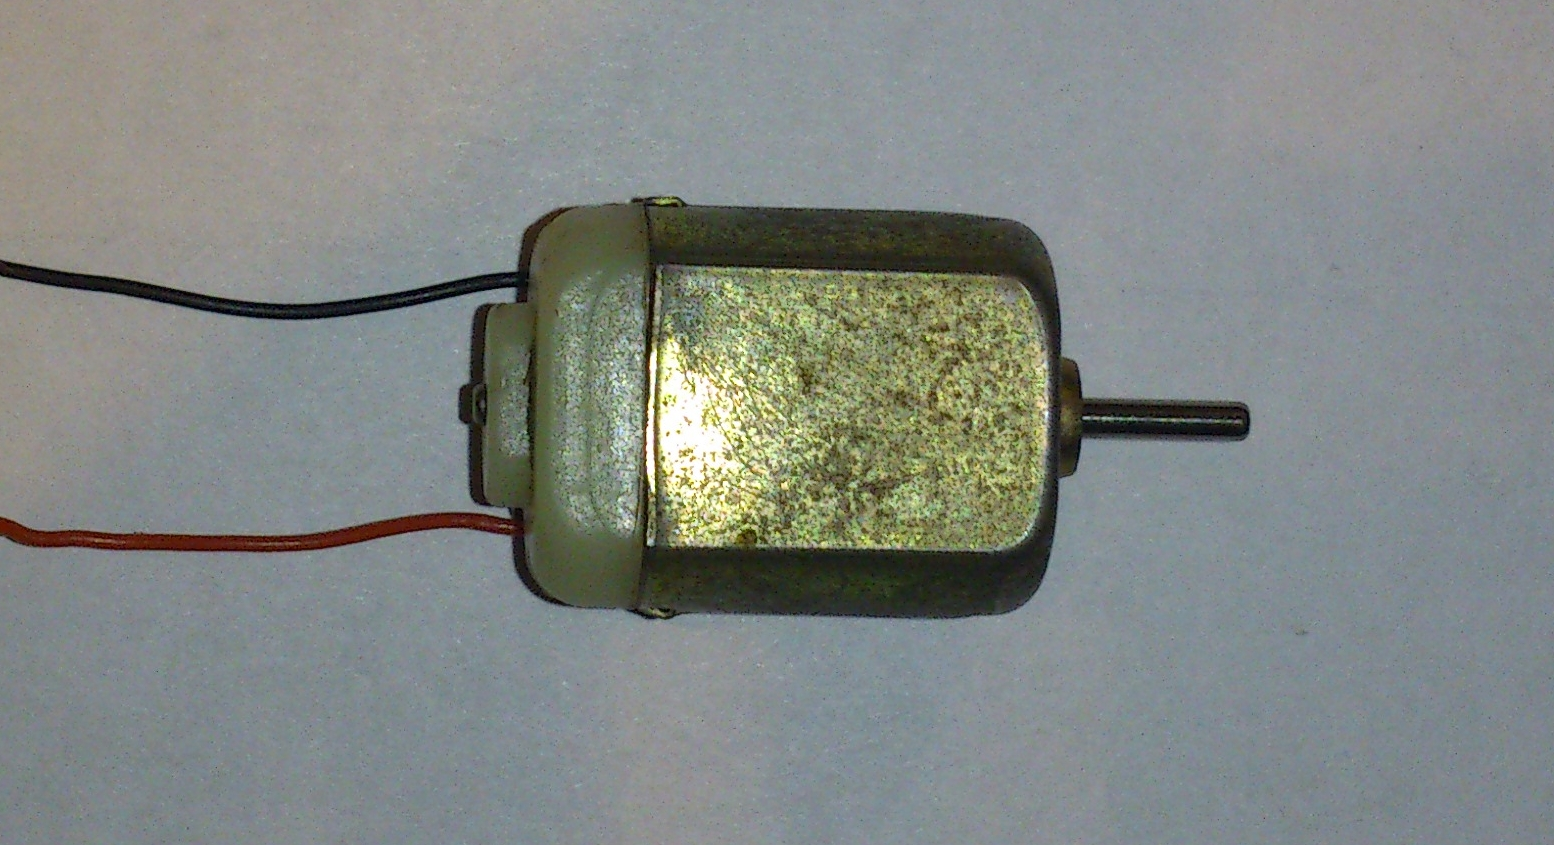
\includegraphics[height = 3 cm]{Media/close_motor.jpg} }
	\end{minipage}
	\hfill
	\begin{minipage}[h]{0.55\linewidth}
		\centering{ 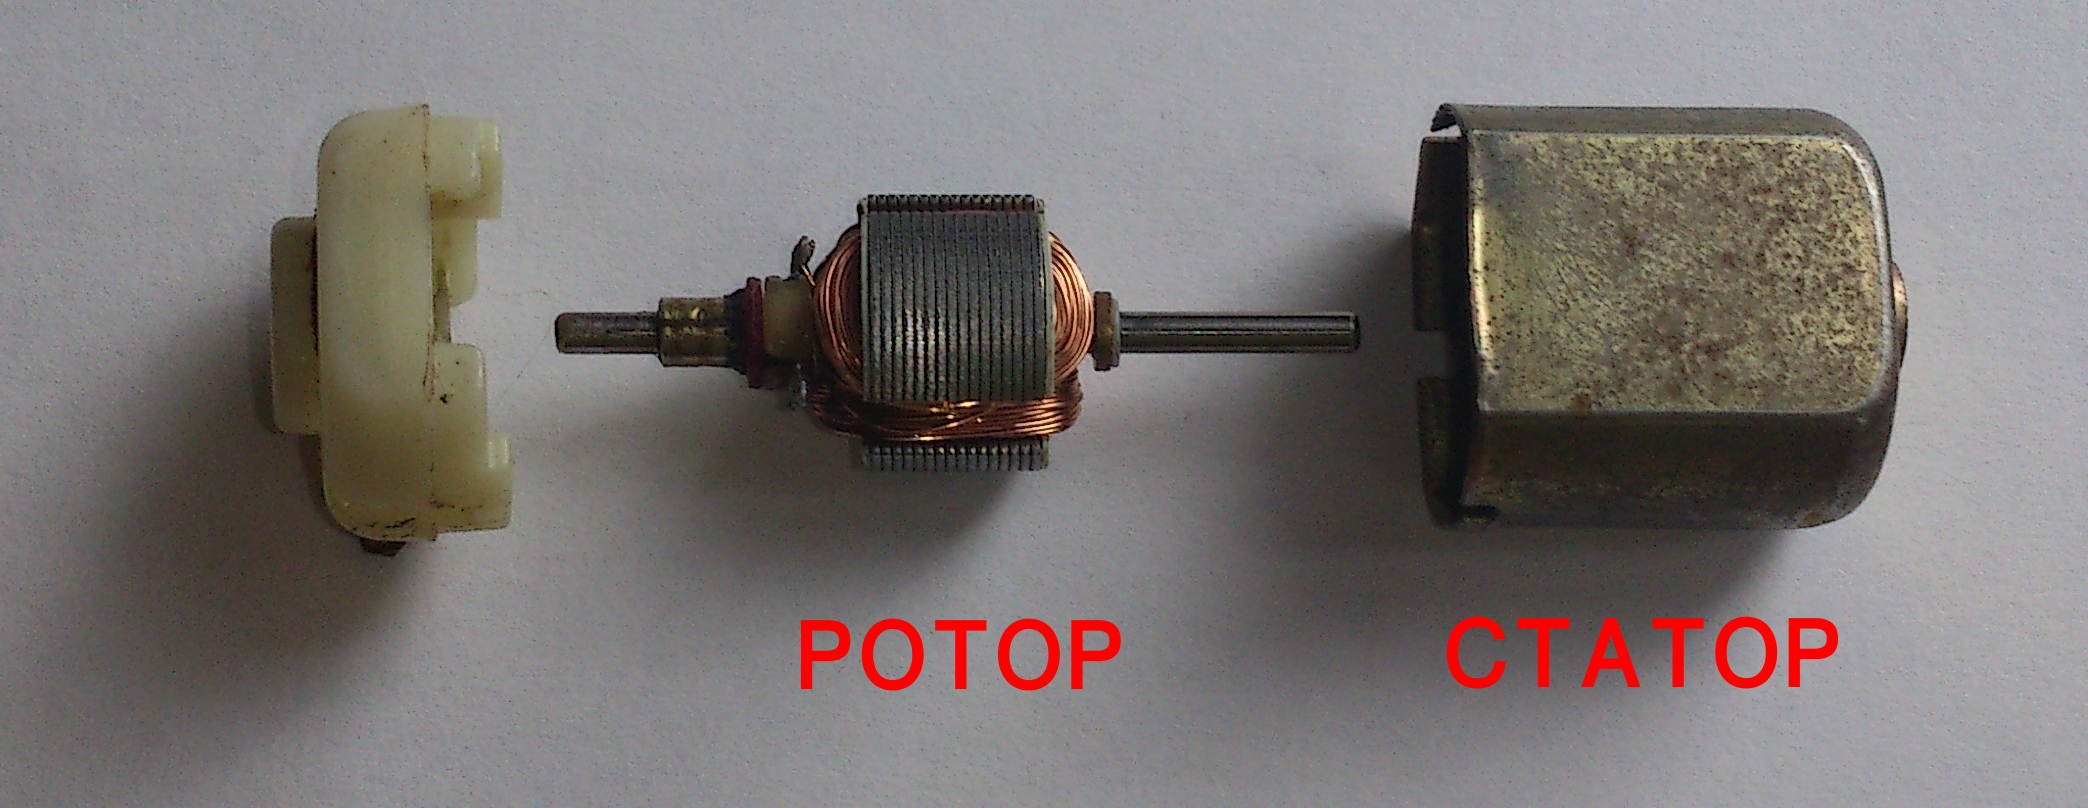
\includegraphics[height = 3 cm]{Media/open_motor.jpg} }
	\end{minipage}
	\caption{Пример двигателя постоянного тока.}
	\label{elmotor}
\end{figure}

Чтобы в дальнейшем было возможно теоретическое рассмотрение исследуемого объекта (двигателя), в первую очередь надо составить \textit{математическую модель} его работы.
Под ней понимается совокупность уравнений, описывающих изменения характеризующих объект величин и их взаимосвязь друг с другом.

С~указанной целью запишем для ротора двигателя второй закон Ньютона в форме, используемой при рассмотрении вращательного движения:
\begin{equation}\label{New's_eq}
	M_\varSigma = J\dot{\omega},
\end{equation}
где $M_\varSigma(t)$~--- сумма всех моментов сил, действующих на ротор; $J$~--- момент инерции ротора\footnote{При рассмотрении вращательного движения тела этот параметр играет ту же роль, что и масса тела при рассмотрении его поступательного движения.}; $\omega(t)$~--- его угловая скорость вращения.
Точкой над буквенным обозначением какой-либо величины здесь и далее будем показывать производную по времени (следовательно $\dot{\omega}$ есть угловое ускорение ротора), а конструкцией, например, $M_\varSigma(t)$~--- тот факт, что $M_\varSigma$ является функцией от времени (для удобства записи формул она может опускаться).

Надо сказать, что составив для упомянутых характеристик двигателя это уравнение, мы уже определили его математическую модель.
Действительно, оно устанавливает связь между всеми величинами, описывающими движение ротора, которые потребуются нам в дальнейшем и тем самым, например, позволяет по известной одной из функций $\dot\omega(t)$ или $M_\varSigma(t)$ найти другую.
Иными словами, благодаря ему появляется возможность прогнозировать поведение ротора двигателя в той или иной ситуации.
Несмотря на это, прежде, чем пойти дальше, скажем еще об одном.

В~данном случае для определения основного уравнения движения ротора двигателя оказалось удобным использование второго закона Ньютона. 
Однако существуют и другие способы нахождения уравнений, описывающих движение механических систем.
Рассмотрим тот из них, который подразумевает использование так называемого {\itshape уравнения Лагранжа второго рода}, записанного с использованием \textit{кинетического потенциала}, и заключается в следующем.

Во-первых, для исследуемой системы записывается {\itshape функция Лагранжа}, или \textit{кинетический потенциал}, которая(-ый) представляет из себя разность её кинетической $T(t)$ и потенциальной $U(t)$ энергий:
\begin{equation}\label{just_lagr}
	L(t) = T - U\ldotp
\end{equation}
Полагая последнюю, которая в рассматриваемой задаче имеет постоянное значение, равной нулю и раскрывая кинетическую энергию вращения ротора по соответствующей формуле, получаем для функции Лагранжа электродвигателя следующее выражение:
\begin{equation}\label{lagr_with_kinet}
	L(t) = T - 0 = \frac{J\dot{\theta}^2}{2}, 
\end{equation}
где $\theta(t)$~--- угол, на который повернулся ротор двигателя из начального положения\lefteqn{.}\footnote{Из определения $\theta(t)$ следует, что $\theta(0) = 0$.}

Необходимо отметить, что в функцию Лагранжа обязательно будут входить некоторые другие функции от времени, характеризующие состояние системы в каждый момент времени~--- так называемые {\itshape обобщённые координаты}, и производные от них~-- {\itshape обобщённые скорости}. 
В~данном случае в роли обобщённой координаты выступает $\theta(t)$.

Во-вторых, для каждой обобщённой координаты и соответствующей ей обобщенной скорости записывается уже упоминаемое уравнение Лагранжа.
Для нашей $\theta(t)$ оно принимает вид
\begin{equation}\label{Lagr's_eq}
	\frac{d}{dt}\frac{\partial L}{\partial\dot\theta}-\frac{\partial L}{\partial\theta} = M_\varSigma(t),
\end{equation}
где, например, конструкцией $\partial L/\partial\theta$ обозначена частная производная от $L$ по $\theta$\lefteqn{,}\footnote{В~данном случае при дифференцировании $L$ по $\theta$, надо принять все переменные кроме $\theta$ постоянными величинами, а $\theta$ той переменной, по которой берется производная. Нижеприведенные примеры должны пояснить сказанное:
\begin{align*}
	\cfrac{\partial\left(3x + 4y\right)}{\partial x} &= 3, & 
	\cfrac{\partial\left(\dfrac{7y^2}{x} + 2y\right)}{\partial y} &= \cfrac{14y}{x} + 2\ldotp
\end{align*}} а конструкцией $d/dt$~--- производная по времени (в данном случае она берется от функции~--- результата операции $\partial L/\partial\dot\theta$). 
При этом в правой части уравнения Лагранжа будет находится некоторая функция, имеющая размерность силы, если обобщённая координата суть линейный размер (например обычная декартова координата), и момента силы, если обобщённая координата~--- некоторый угол.
Эта функция называется \textit{обобщенной силой}.
На данный момент под ней следует понимать просто сумму всех действующих в системе сил или моментов сил, которые вызывают изменение рассматриваемой обобщенной координаты.
В~действительности сказанное неверно\lefteqn,\footnote{Все моменты сил, действующие на якорь, которые мы будем рассматривать в дальнейшем, допускают указанное упрощение, поэтому в правой части уравнения~\eqref{Lagr's_eq} и стоит $M_\varSigma$ без каких-либо изменений.} однако описание точных правил определения обобщенных сил мы оставим для следующих лабораторных.

После написания уравнения остается только взять необходимые производные, что мы и сделаем.
 
Так как в функции Лагранжа~\eqref{lagr_with_kinet} нет членов включающих $\theta$, второе слагаемое можно отбросить\lefteqn{.}\footnote{Производная от постоянной равна нулю.} 
Тогда уравнение~\eqref{Lagr's_eq} с учётом~\eqref{lagr_with_kinet} запишется в виде
\begin{equation}\label{Lagr's_eq_without_last}
	M_\varSigma = \frac{d}{dt}\Biggl(\frac{\partial}{\partial\dot\theta}\biggl(\!\frac{J\dot{\theta}^2}{2}\biggr)\Biggr)\ldotp
\end{equation}
Выполнив дифференцирование по $\dot\theta$, будем иметь
\begin{equation} \label{after_first_dif}
	M_\varSigma = \frac{d}{dt}\left(\!J\dot\theta\right)\!,
\end{equation}
и взяв производную по времени, получим окончательный результат:
\begin{equation} \label{after_sec_dif}
	M_\varSigma = J\ddot\theta\ldotp
\end{equation}

Если теперь ввести обозначение $\omega = \dot\theta$, станет очевидно, что найденное данным методом уравнение совпадает с тем, которое было  получено с помощью второго закона Ньютона~\eqref{New's_eq}. 
Таким образом, мы показали, что оба метода эквивалентны. 
Использованию уравнения Лагранжа ещё будут посвящены следующие занятия, а теперь продолжим дальнейшее изучение работы двигателя.
 
\paragraph*{Пример применения математической модели}$\phantom{-}$\\
\hspace*{\parindent}С~помощью найденной математической модели установим зависимость $\omega(t)$, которая выполняется при разгоне из состояния покоя ненагруженного ротора двигателя при подаче на него постоянного напряжения.

Как уже было сказано, для того чтобы это действие было возможным, необходимо знать зависимость $M_\varSigma(t)$, поэтому сначала определим, как в данном процессе выглядит она.

Величину $M_\varSigma$ можно представить суммой двух слагаемых:
\begin{equation}
	M_\varSigma = M_{el} + M_{oth},
\end{equation}
где $M_{el}$~--- момент силы, возникающий в двигателе из-за протекающих в нем электродинамических процессов и раскручивающий его якорь; $M_{oth}$~--- сумма всех остальных моментов сил\lefteqn{,}\footnote{В качестве примера таковых можно привести моменты сил трения и моменты, создаваемые весами каких-либо конструктивных элементов, прикрепленных к валу ротора.} действующих на ротор.
Поскольку мы рассматриваем ситуацию, когда якорь двигателя ничем не нагружен и полагаем силы трения отсутствующими, то 
\begin{equation}
	M_{oth} = 0,
\end{equation} 
а значит 
\begin{equation}
	M_\varSigma = M_{el},
\end{equation}
то есть ранее поставленная задача сводится к нахождению вида функции $M_{el}(t)$.

Вращающий момент $M_{el}$ несложно определить, если предположить его пропорциональным действующей в цепи двигателя ЭДС ($U_{cv}$)\footnote{На на следующем занятии будет показано, что при определенных условиях это предположение полностью оправдывается.}:
\begin{equation}\label{connect_M_U}
	M_{el} = \alpha_1U_{cv},
\end{equation}
где $\alpha_1$~--- некоторая постоянная.
В~этом случае можно сказать следующее.
  
В~начальный момент времени, когда мы только подали напряжение на двигатель, а ротор ещё не пришел в движение, момент силы $M$ принимает некоторое значение $M_{st}$, которое в дальнейшем мы будем называть {\itshape пусковым моментом}, равное 
\begin{equation}\label{M_pusk}
	M_{st}=\alpha_1U_{ctrl},
\end{equation}
где $U_{ctrl} = const$~--- ЭДС источника электрической энергии, например аккумулятора, (в самом начале создавать $U_{cv}$ будет только она).  
В~последующие моменты времени из-за вращения ротора в его катушках возникнет ЭДС индукции, направленная против $U_{ctrl}$ и прямопропорциональная угловой скорости вращения ротора\footnote{Это равенство также будет доказано на следующем занятии.}:
\begin{equation}\label{connect_w_E}
	\mathcal E_i(\omega)=\alpha_2\omega,
\end{equation}  
где $\alpha_2$~--- некоторая постоянная. 
При этом суммарная ЭДС в цепи будет равняться
\begin{equation}\label{connect_of_U}
	U_{cv}=U_{ctrl}-\mathcal E_i
\end{equation} 
и, следовательно, будет уменьшаться. 
Согласно выражению~\eqref{connect_M_U}, уменьшаться будет и момент силы, причем, подставив значение для $U_{cv}$ из~\eqref{connect_M_U}, выражение для $\mathcal E_i$ из~\eqref{connect_w_E} и значение для $U_{ctrl}$ из~\eqref{M_pusk} в уравнение~\eqref{connect_of_U}, мы найдем зависимость $M_{el}(\omega)$, которая при этом выполняется:
\begin{equation*}\label{bad_M(w)*}
	\frac{M_{el}}{\alpha_1}=\frac{M_{st}}{\alpha_1}-\alpha_2\omega\ldotp
\end{equation*}
Отсюда окончательно имеем, что
\begin{equation}\label{bad_M(w)}
	M_{el}(\omega)=M_{st}-\alpha_1\alpha_2\omega\ldotp
\end{equation}

Значение неизвестной постоянной (произведения $\alpha_1\alpha_2$), входящей в полученное уравнение, можно определить из условия о том, что при достижении ротором двигателя максимальной скорости вращения $\omega_{nls}$ (согласно опытным данным, двигатель не разгоняется бесконечно долго) действующий на него момент силы $M_{el}$ обращается в нуль. 
Если предположить, что это не так (момент будет отличен от нуля), получается, что на ротор будут продолжать действовать разгоняющие его силы, а значит, он будет ускоряться, что, в свою очередь, неверно. 
Одним словом, при достижении ротором скорости вращения $\omega_{nls}$ выражение~\eqref{bad_M(w)} принимает вид
\begin{equation*}\label{M(w0)}
	0 = M_{st} - \alpha_1\alpha_2\omega_{nls},
\end{equation*} 
откуда имеем, что
\begin{equation}\label{a1a2}
	\alpha_1\alpha_2 = \frac{M_{st}}{\omega_{nls}}\ldotp
\end{equation}
С~учетом этого выражения зависимость~\eqref{bad_M(w)} примет более удобную для использования форму:
\begin{equation}\label{M(w)}
	M_{el}(\omega) = M_{st} - \frac{M_{st}}{\omega_{nls}}\,\omega,
\end{equation}
так как все входящие в выражение~\eqref{M(w)} величины имеют ясный физический смысл.

Получившееся уравнение и есть искомая зависимость $M_\varSigma(t)$\lefteqn{.}\footnote{В~данном случае мы имеем дело со сложной функцией от времени $M_\varSigma\bigl(\omega(t)\bigr)$.}
Теперь, для того чтобы окончательно решить поставленную задачу о нахождении зависимости скорости вращения ротора от времени ($\omega(t)$), остается лишь заменить $M_\varSigma$ в выражении~\eqref{New's_eq} соотношением~\eqref{M(w)} и решить получившееся дифференциальное уравнение\footnote{Дифференциальным называется уравнение, связывающее искомую функцию (в данном случае $\omega(t)$), её производные и аргумент некоторым соотношением.}:
\begin{equation}\label{diffur}
	M_{st} - \omega\frac{M_{st}}{\omega_{nls}} = J\dot\omega \qquad \Rightarrow \qquad 
	\frac{M_{st}}{\omega_{nls}}(\omega_{nls} - \omega) = J\frac{d\omega}{dt}\ldotp
\end{equation}

Приведем его решение.

Сначала умножим обе его части на~$dt$, а потом разделим на выражение в скобках и на $J$:
\begin{equation}
	\frac{M_{st}}{J\omega_{nls}}dt=\frac{d\omega}{\omega_{nls}-\omega}\ldotp
\end{equation}
Проинтегрируем обе части выражения, в результате чего получим
\begin{equation}
	\frac{M_{st}}{J\omega_{nls}}\,t=-\ln |\omega_{nls}-\omega|+C\ldotp
\end{equation}
В~нашем случае $\omega_{nls}>\omega$, поэтому знак модуля можно просто опустить. 
Перепишем неизвестную постоянную $C$ в виде $-\ln C_1$, тогда получим
\begin{equation}
	\frac{M_{st}}{J\omega_{nls}}\,t=-\ln(\omega_{nls}-\omega)-\ln C_1\ldotp
\end{equation}
Заменив сумму логарифмов логарифмом произведения, потенцированием избавимся от натурального логарифма:
\begin{equation}\label{not_yet}
	\exp\!\left(-\frac{M_{st}}{J\omega_{nls}}t\right)=C_1(\omega_{nls}-\omega)\ldotp
\end{equation}
Из начальных условий~--- в момент времени $t=0$ скорость равна нулю $\omega=0$~--- определим $C_1$:
\begin{equation}
	\exp(0)=C_1(\omega_{nls}-0) \qquad \Rightarrow \qquad C_1=\frac{1}{\omega_{nls}}\ldotp
\end{equation}
С~учетом этого значения получим из~\eqref{not_yet} окончательное решение:
\begin{equation}\label{w(t)}
	\omega(t)=\omega_{nls}\left(1-\exp\Bigl(-\frac{M_{st}}{J\omega_{nls}}t\Bigr)\right)\ldotp
\end{equation}

Проанализировав это выражение, можно сказать, что характер зависимости $\omega(t)$ определяется значениями таких величин, как максимальная скорость вращения ротора, пусковой момент и момент инерции ротора, а её график имеет вид, представленный на рис.~\ref{graph_w(t)}. 

\begin{figure}[h]
	\noindent\centering{
		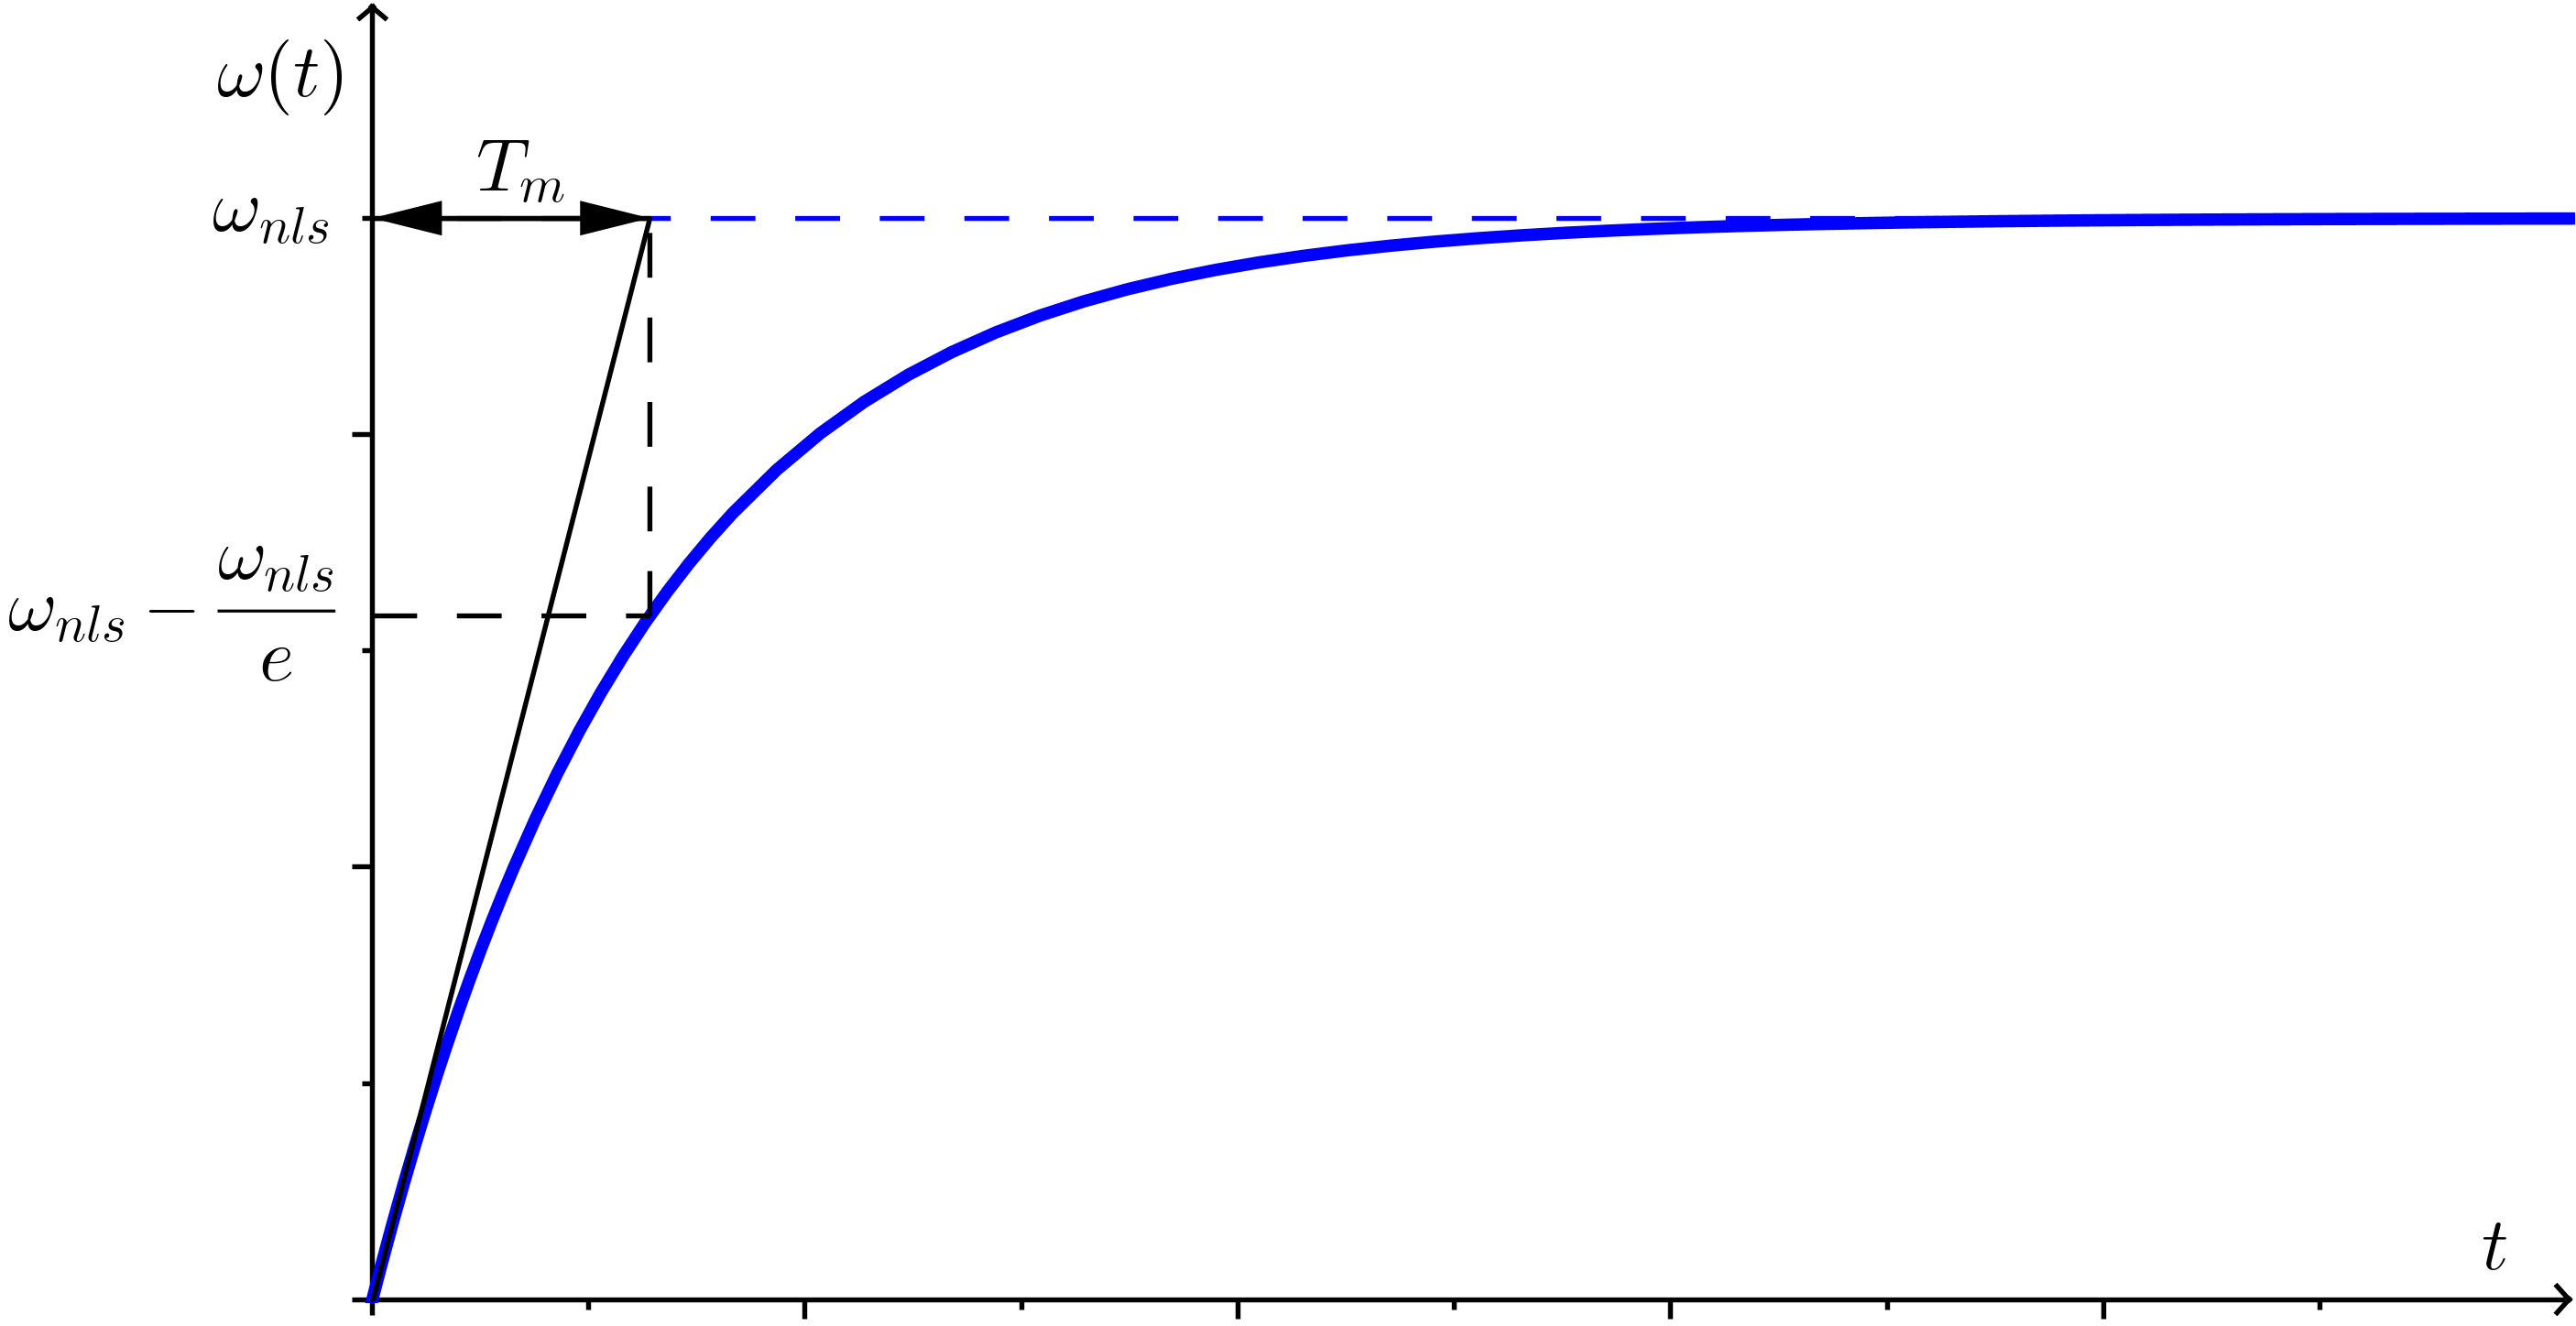
\includegraphics[scale=1.1]{Media/graph_w(t)_en.png}
	}
	\caption{График зависимости угловой скорости вращения ротора от времени.}
	\label{graph_w(t)}
\end{figure}

Уравнение~\eqref{w(t)} можно записать, используя еще одну величину, характеризующую двигатель постоянного тока~--- электромеханическую постоянную времени $T_m$, равную
\begin{equation}\label{T_m}
	T_m = \cfrac{J\omega_{nls}}{M_{st}}\,\ldotp
\end{equation}
Тогда уравнение~\eqref{w(t)} примет вид:
\begin{equation}
	\omega(t) = \omega_{nls}\left(1 - \exp\left(-\frac{t}{T_m}\right)\right),
\end{equation} 
откуда нетрудно определить физический смысл величины $T_m$: она есть время, за которое скорость вращения первоначально покоящегося ротора возрастает до 
\begin{equation}
	\omega(T_m) = \omega_{nls} - \frac{\omega_{nls}}{e}\ldotp
\end{equation}

%Определить значение $T_m$ можно делением значения максимальной скорости вращения $\omega_{nls}$ на производную от зависимости $\omega(t)$ в точке нуль, в которой она равна\footnote{Cамостоятельно убедитесь, что это именно так.}
%\begin{equation}\label{w'(0)}
%	\dot\omega(0) = \frac{M_{st}}{J}\ldotp
%\end{equation} 

Таким образом, мы решили ранее поставленную задачу, определив c помощью математической модели закон изменения скорости вращения ротора двигателя от времени, однако прежде, чем закончить данный раздел, получим из найденной зависимости выражения для углового ускорения якоря двигателя ($\varepsilon$) и для его угловой координаты ($\theta$):
\begin{gather}
	\varepsilon(t) = \dot\omega = \frac{\omega_{nls}}{T_m}\exp\Bigl(-\frac{t}{T_m}\Bigr),\\
	\theta(t) = \int\!\omega\,dt = \omega_{nls}t + \omega_{nls}T_m\exp\Bigl(-\frac{t}{T_m}\Bigr) + C_2,
\end{gather}
где $C_2$~--- некоторая постоянная, чье значение можно определить из начальных условий ($\theta(0) = 0$):
\begin{equation}
	\theta(0) = \omega_{nls}\cdot0 + \omega_{nls}T_m\exp\Bigl(-\frac0{T_m}\Bigr) + C_2 \qquad \Rightarrow \qquad C_2 = -\omega_{nls}T_m
\end{equation}
С учетом найденного значения постоянной $C_2$ окончательно имеем:
\begin{gather}
	\varepsilon(t) = \frac{\omega_{nls}}{T_m}\exp\Bigl(-\frac{t}{T_m}\Bigr),\\
	\theta(t) = \omega_{nls}\Biggl(t - T_m\biggl(1 - \exp\Bigl(-\frac{t}{T_m}\Bigr)\biggr)\Biggr),\label{theta(t)}
\end{gather}
и графики, показанные на рис.~\ref{graphs}.

\begin{figure}[h]
	\begin{minipage}[h]{0.44\linewidth}
		\center{ 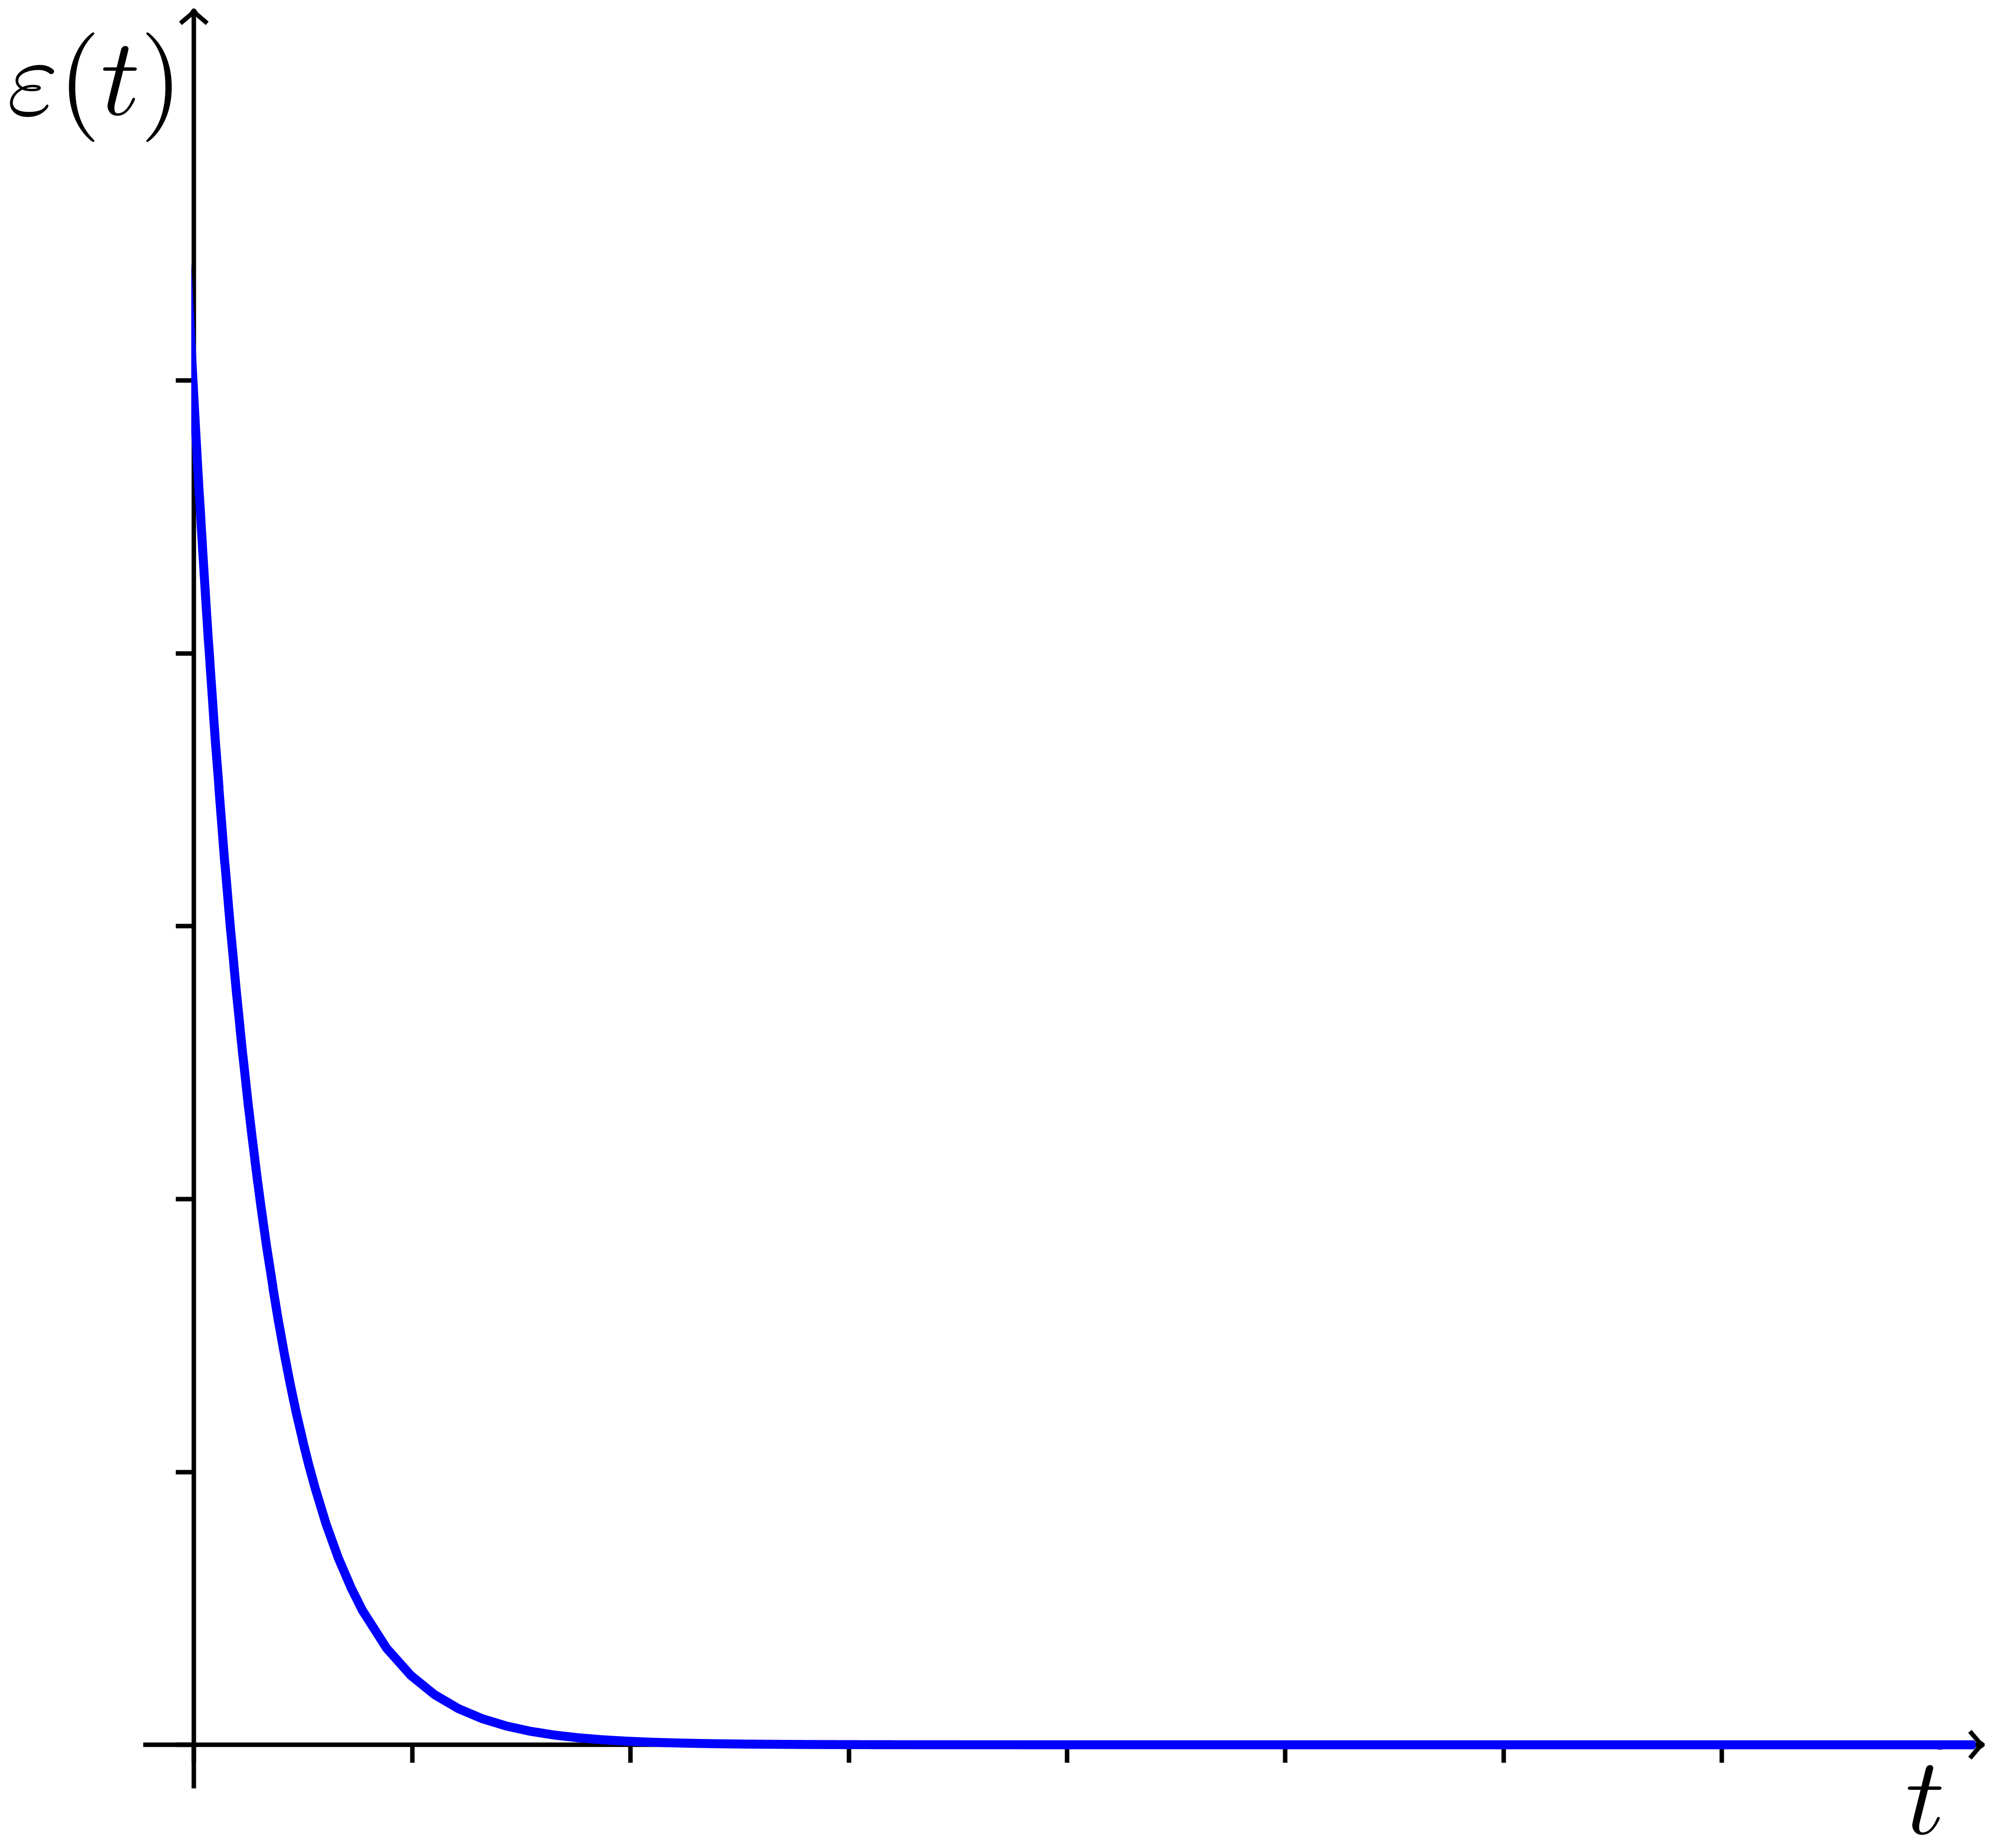
\includegraphics[height = 6 cm]{Media/e(t).png} }
	\end{minipage}
	\hfill
	\begin{minipage}[h]{0.55\linewidth}
		\centering{ 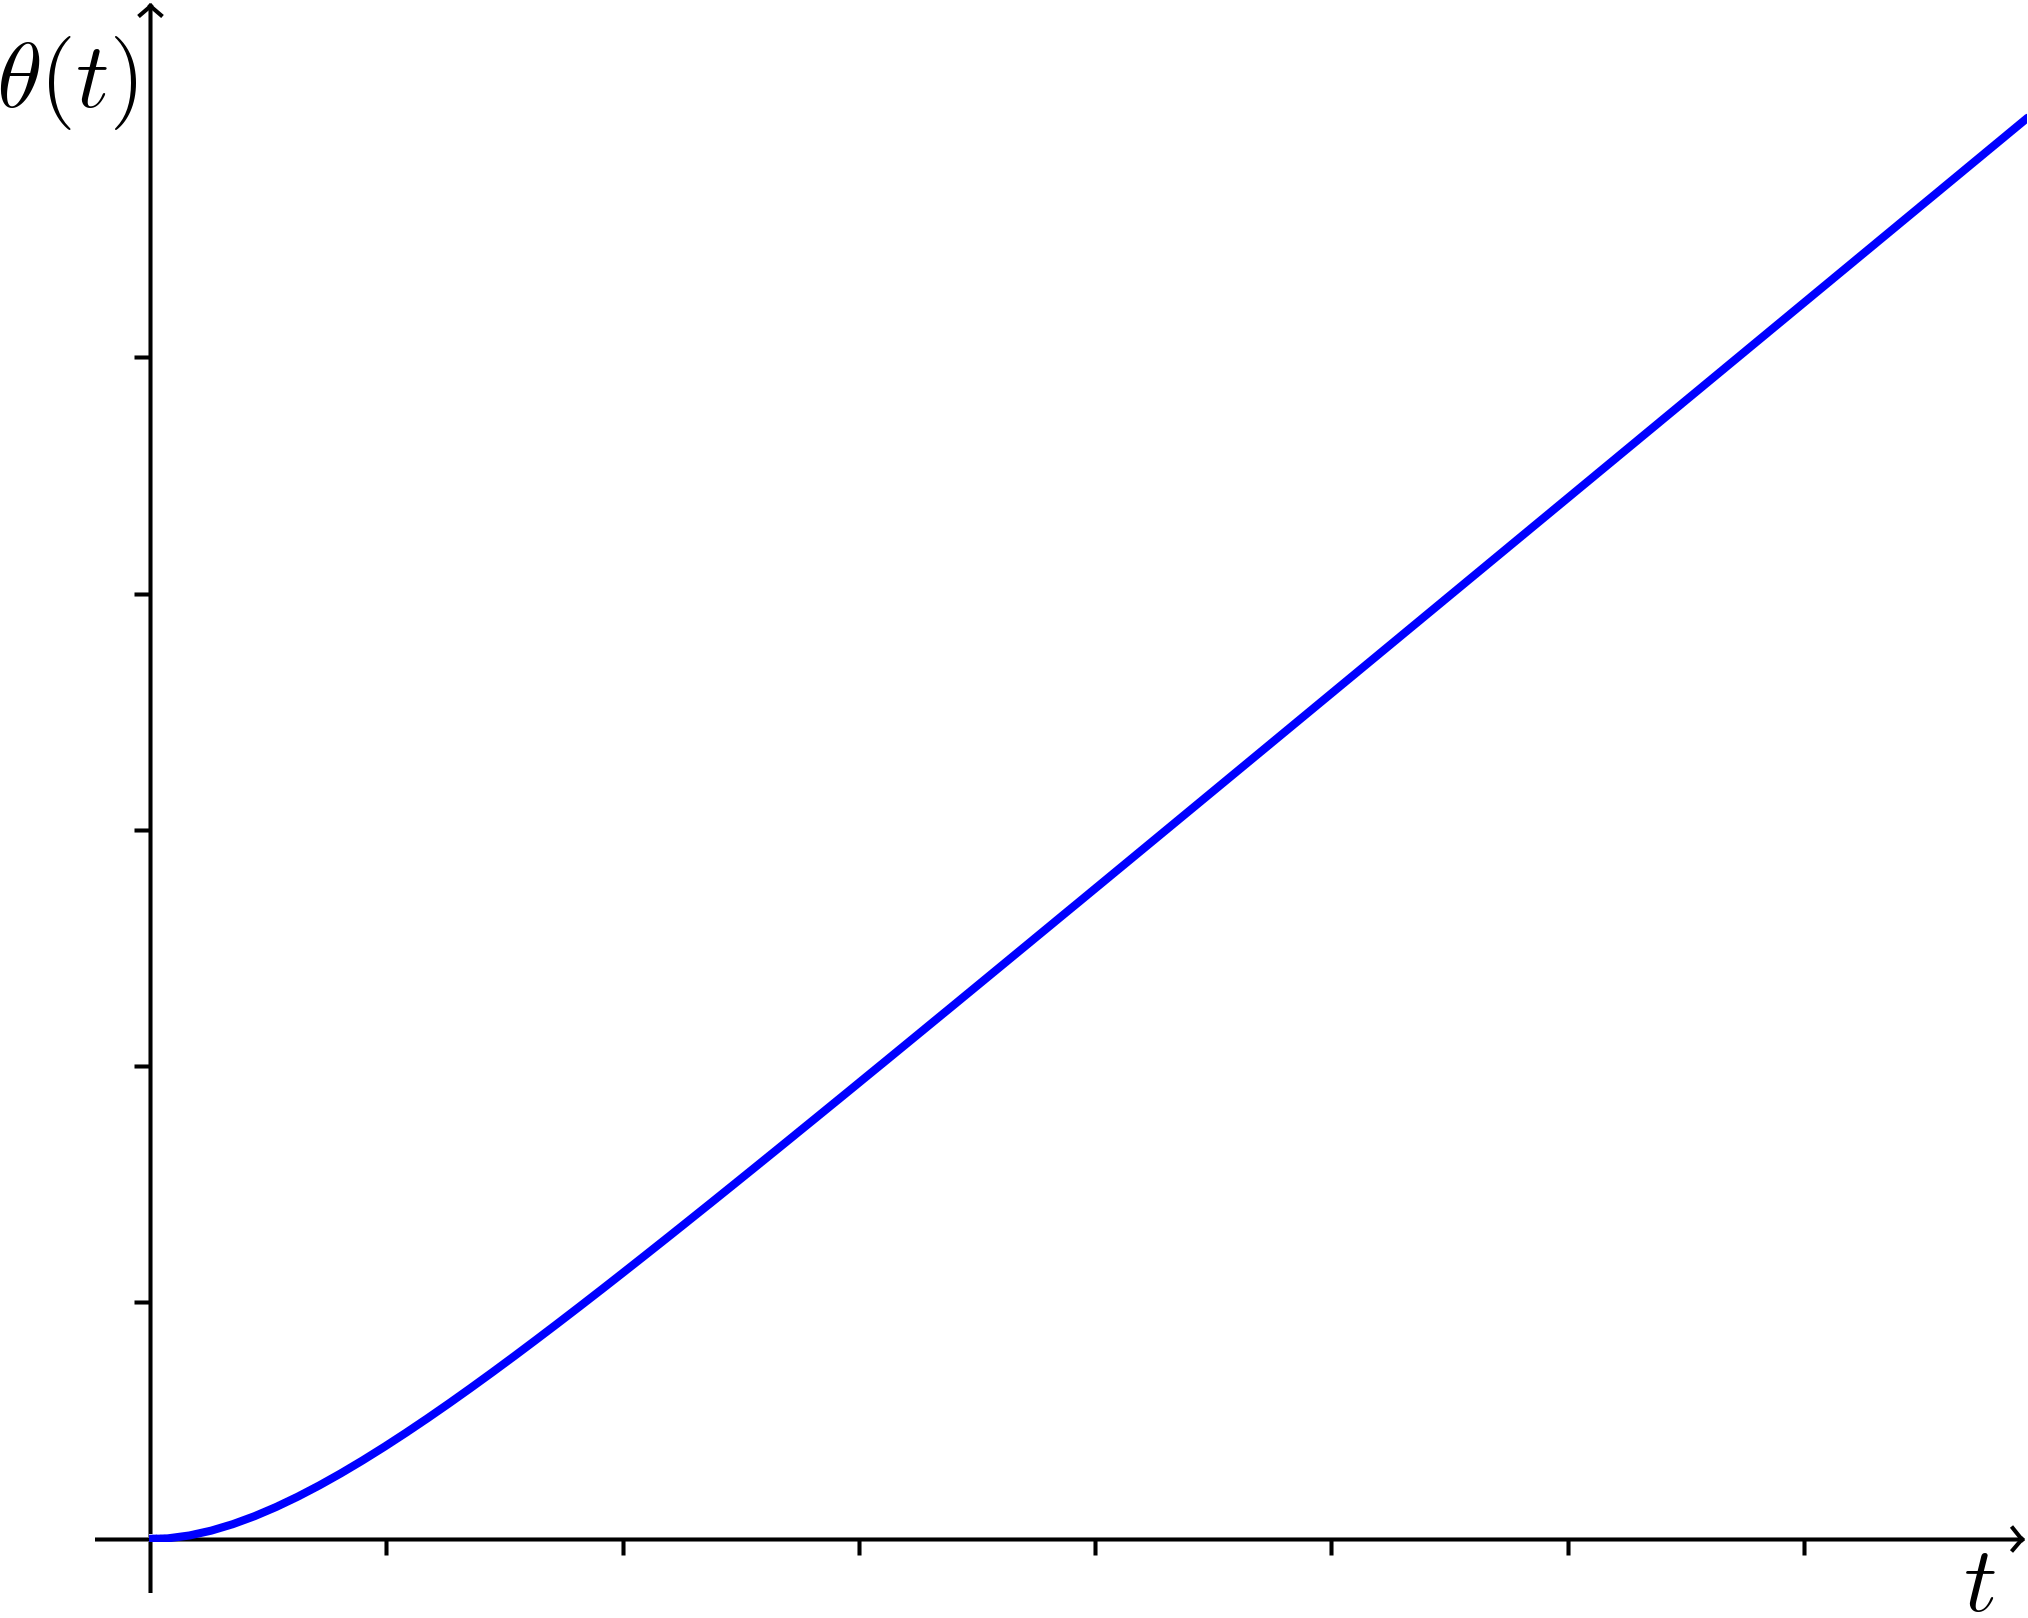
\includegraphics[height = 6 cm]{Media/th(t).png} }
	\end{minipage}
	\caption{Графики зависимостей $\varepsilon(t)$ и $\theta(t)$.}
	\label{graphs}
\end{figure}
	
Целью практической части данной работы и будет опытная проверка результатов, полученных в этом разделе. 


%В~технических задачах, связанных с автоматическим управлением, все явления, например движение тел или изменение их температуры, рассматриваются как некоторые {\itshape процессы}. 
%Каждый из них прежде всего характеризуется:
%\begin{itemize}
%\item {\itshape входными сигналами}~--- величинами, которые приводят к изменению текущего состояния системы и с помощью которых, следовательно, осуществляется управление;
%\item {\itshape выходными сигналами}~--- величинами, которые характеризуют состояние системы в данный момент времени и над которыми, соответственно, осуществляется управление;
%\item функциональной зависимостью между ними~--- грубо говоря, информацией о том, как входные сигналы изменяют выходные.
%\end{itemize}   
%В~связи с этим применяют еще один способ представления принципов работы исследуемых систем, который в отличие от аналитического (использующего формулы, до сих пор мы пользовались именно им) отражает все эти характеристики более наглядно. 

\paragraph*{Моделирование работы двигателя}$\phantom{-}$\\
\hspace*{\parindent}Для того чтобы получать из математической модели количественную информацию о рассматриваемом процессе, необязательно прибегать к решению дифференциальных уравнений.
Например, с указанной задачей успешно справляются ряд вычислительных программ, подобных Scilab Xcos, которую мы будем использовать в данном курсе.
При этом суть требуемой работы в таком случае оказывается следующей. 

Во-первых, на основании составленной математической модели исследуемого процесса в упомянутых программах строится блок-схема, описывающая единичный такт циклически повторяющихся математических операций, соответствующих изменению характеризующих процесс величин.
К слову сказать, созданная в Xcos на основании уравнения~\eqref{diffur} для ранее рассмотренного нами разгона ненагруженного двигателя эта схема будет выглядеть так, как показано на рис.~\ref{struct_sheme}\lefteqn{.}\footnote{Некоторые несущественные детали схемы такие, как, например, форма некоторых блоков, в зависимости от используемого программного обеспечения и его версий могут различаться.}
Во-вторых, по полученной схеме производится моделирование процесса и непосредственно сбор всех интересующих исследователя данных.

\begin{figure}[h]
	\noindent\centering{
		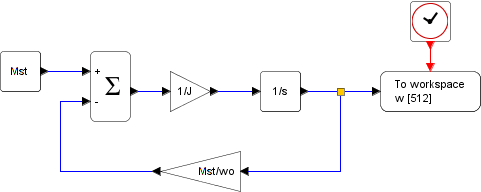
\includegraphics[scale=0.8]{Media/struct_sheme_white.png}
	}
	\caption{Схема моделирования исследуемого процесса.}
	\label{struct_sheme}
\end{figure}

Для раскрытия принципов работы данного подхода скажем следующее.

Каждый блок, составляющий схему имеет в своем составе {\itshape входы} и {\itshape выходы}, обозначенные треугольничками, направленными соответственно в тело блока и от него. 
Общение блоков осуществляется с помощью сигналов~--- определенных числовых значений. 
Последние, перемещаясь по каналам связи (обозначены синими и красными линиями), приходят на вход блока, в нем изменяются и уже в измененной форме поступают на его выход для дальнейшего путешествия по каналам связи. 

Начинающий эту схему блок с буквенным обозначением <<Mst>> и с одним выходом означает, что на последний подается значение, хранящееся в переменной Mst (очевидно, что ей надо присвоить значение, равное $M_{st}$). 
Блоки в форме треугольника умножают входящий сигнал на значение написанного на себе выражения и подают полученный результат на выход. 
Блок со значком суммы ($\sum$) вычитает из своего сигнала, идущего на вход, помеченный знаком <<$+$>>, другой сигнал (идущий на вход, помеченный знаком <<$-$>>) и подает на свой выход значение этой разности.
Блок с надписью <<1/s>> интегрирует входной сигнал и прибавляет к числовому значению, хранящемуся в его памяти\lefteqn{.}\footnote{Имеется в виду следующее. Как известно, определенный интеграл дает лишь приращение первообразной $F(x)$ своей функции-<<аргумента>> $f(x)$, то есть:
\begin{equation}
	\int_a^b\! f(x)\,dx = F(b) - F(a)\ldotp
\end{equation}
При таком условии, для того чтобы иметь возможность вычислять именно значение первообразной в интересующей точке $x = b$, надо знать ее значение в начальной точке $x = a$:
\begin{equation}
	F(b) = \int_a^b\! f(x)\,dx + F(a)\ldotp
\end{equation}

Возможность помещать в память интегратора постоянное числовое значение как раз и рассчитана на то, что в качестве такого будет взято $F(a)$, ведь в этом случае, согласно сказанному, данный блок будет выдавать значение $F(b)$.}
Эта сумма потом поступает на его выход.
Остальные два блока~--- с изображением часов и с фразой <<To workspace>>~--- нужны лишь для того, чтобы сохранить результаты моделирования, отнесенные к заданным промежуткам времени, в используемой среде разработки.

Теперь же покажем, как данная схема расшифровывается (читается). 
На блок-сумматор (тот, который помечен значком $\sum$), приходят два сигнала: один поступает из блока с надписью <<Mst>> и несет значение, равное пусковому моменту, второй~--- с конца схемы (выхода интегратора) и заключает в себе хранящееся в его памяти число\lefteqn{,}\footnote{Забегая вперед, можно сказать, что в результате моделирования нашей схемы мы хотим получить числовые данные для зависимости $\omega(t)$. Поскольку в начале рассматриваемого процесса скорость ротора равна нулю, то и в память данного блока следует поместить $0$.}  умноженное нижним блоком-треугольником на $M_{st}/\omega_{nls}$.
Эти сигналы вычитаются друг из друга, и полученная разность приходит на следующий блок, где умножается на значение $1/J$.
В~таком виде она идет дальше.
Таким образом, на блок с надписью <<1/s>> поступает значение, равное $M_{st}/J$, которое после интегрирования, согласно~\eqref{diffur}, даст не что иное, как некоторое значение угловой скорости вращения ротора $\omega_1$ в <<первый>> момент времени\lefteqn{.}\footnote{Каждый обход схемы сигналами осуществляется через равные промежутки времени, длительность которых можно задавать вручную. По указанной причине первое прохождение схемы и полученные в результате его числовые результаты будут отнесены к моменту времени, равному $t = \tau$, где $\tau$~--- упомянутая временная задержка. Следующий обход~--- к $t = 2\tau$ и т.д. Моменту времени $t = 0$ будет соответствовать сигнал находящийся в конце схемы при ее запуске.}
Этот сигнал, в свою очередь, пойдет в память среды Xcos и, будучи умноженным на $M_{st}/\omega_{nls}$, на один из входов сумматора. 
С~учетом этого имеем, что при втором и последующих обходах сигналами схемы на выходе последнего будет формироваться значение $M_{st}-\omega_i M_{st}/\omega_{nls}$, где $\omega_i$~--- скорость, вычисленная в предыдущем цикле. 
Это значение, поделенное на $J$ и после этого проинтегрированное, согласно~\eqref{diffur}, опять даст значение скорости $\omega_{i+1}$, но уже в другой момент времени~--- следующий за тем, в течение которого скорость была равна $\omega_i$.  

Так повторяясь много раз, данный процесс сформирует два массива данных, в первом из которых будут находиться значения скорости~--- значения сигналов, пришедших на вход блока с надписью <<To workspace>> со стороны схемы, а во втором~--- соответствующие моменты времени, которые представляют из себя значения сигналов, поступивших в этот блок со стороны <<часов>>.
Построенный по их данным график в случае, если схема была построена правильно, совпадет с графиком функции~\eqref{w(t)}~--- см.~рис.~\ref{graph_w(t)}.

В~заключение сделаем два замечания.
Во-первых, те численные значения, с которыми блоками приходится иметь дело, в используемом в рамках данного курса ПО можно задавать и в явном виде, а не через переменные.
С~учетом этого схема моделирования двигателя может выглядеть и как на рис.~\ref{struct_sheme_chisl}.
\begin{figure}[h]
	\noindent\centering{
		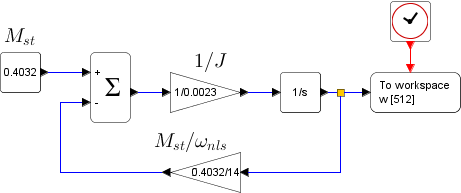
\includegraphics[scale=1]{Media/struct_sheme_chisl.png}
	}
	\caption{Схема процесса, возвращающая значения зависимости $\omega(t)$.}
	\label{struct_sheme_chisl}
\end{figure}
Во-вторых, если добавить в конце схемы процесса еще один интегратор (рис.~\ref{struct_sheme_theta}), то на его выходе будут формироваться значения угловой координаты поворота якоря ($\theta$).
\begin{figure}[h]
	\noindent\centering{
		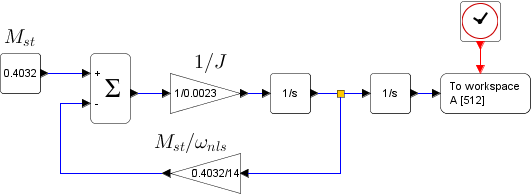
\includegraphics[scale=1]{Media/struct_sheme_theta.png}
	}
	\caption{Схема процесса, возвращающая значения зависимости $\theta(t)$.}
	\label{struct_sheme_theta}
\end{figure}

\newpage
\section{Цель работы}
\hspace*{\parindent}Познакомиться с оборудованием и программным обеспечением, которые понадобятся при изучении материала данного курса.
Экспериментально проверить истинность найденных функций, описывающих работу ненагруженного двигателя постоянного тока, и определить значения входящих в них параметров $\omega_{nls}$ и $T_m$.  

\section{Порядок выполнения работы}
\begin{enumerate}
\item Снятие показаний с двигателя EV3\\(при возникновении вопросов попробуйте обратиться к Приложению А).
\begin{enumerate}
\item Соберите конструкцию, показанную на рис.~\ref{brick}.\\
\begin{figure}[h]
	\noindent\centering{
		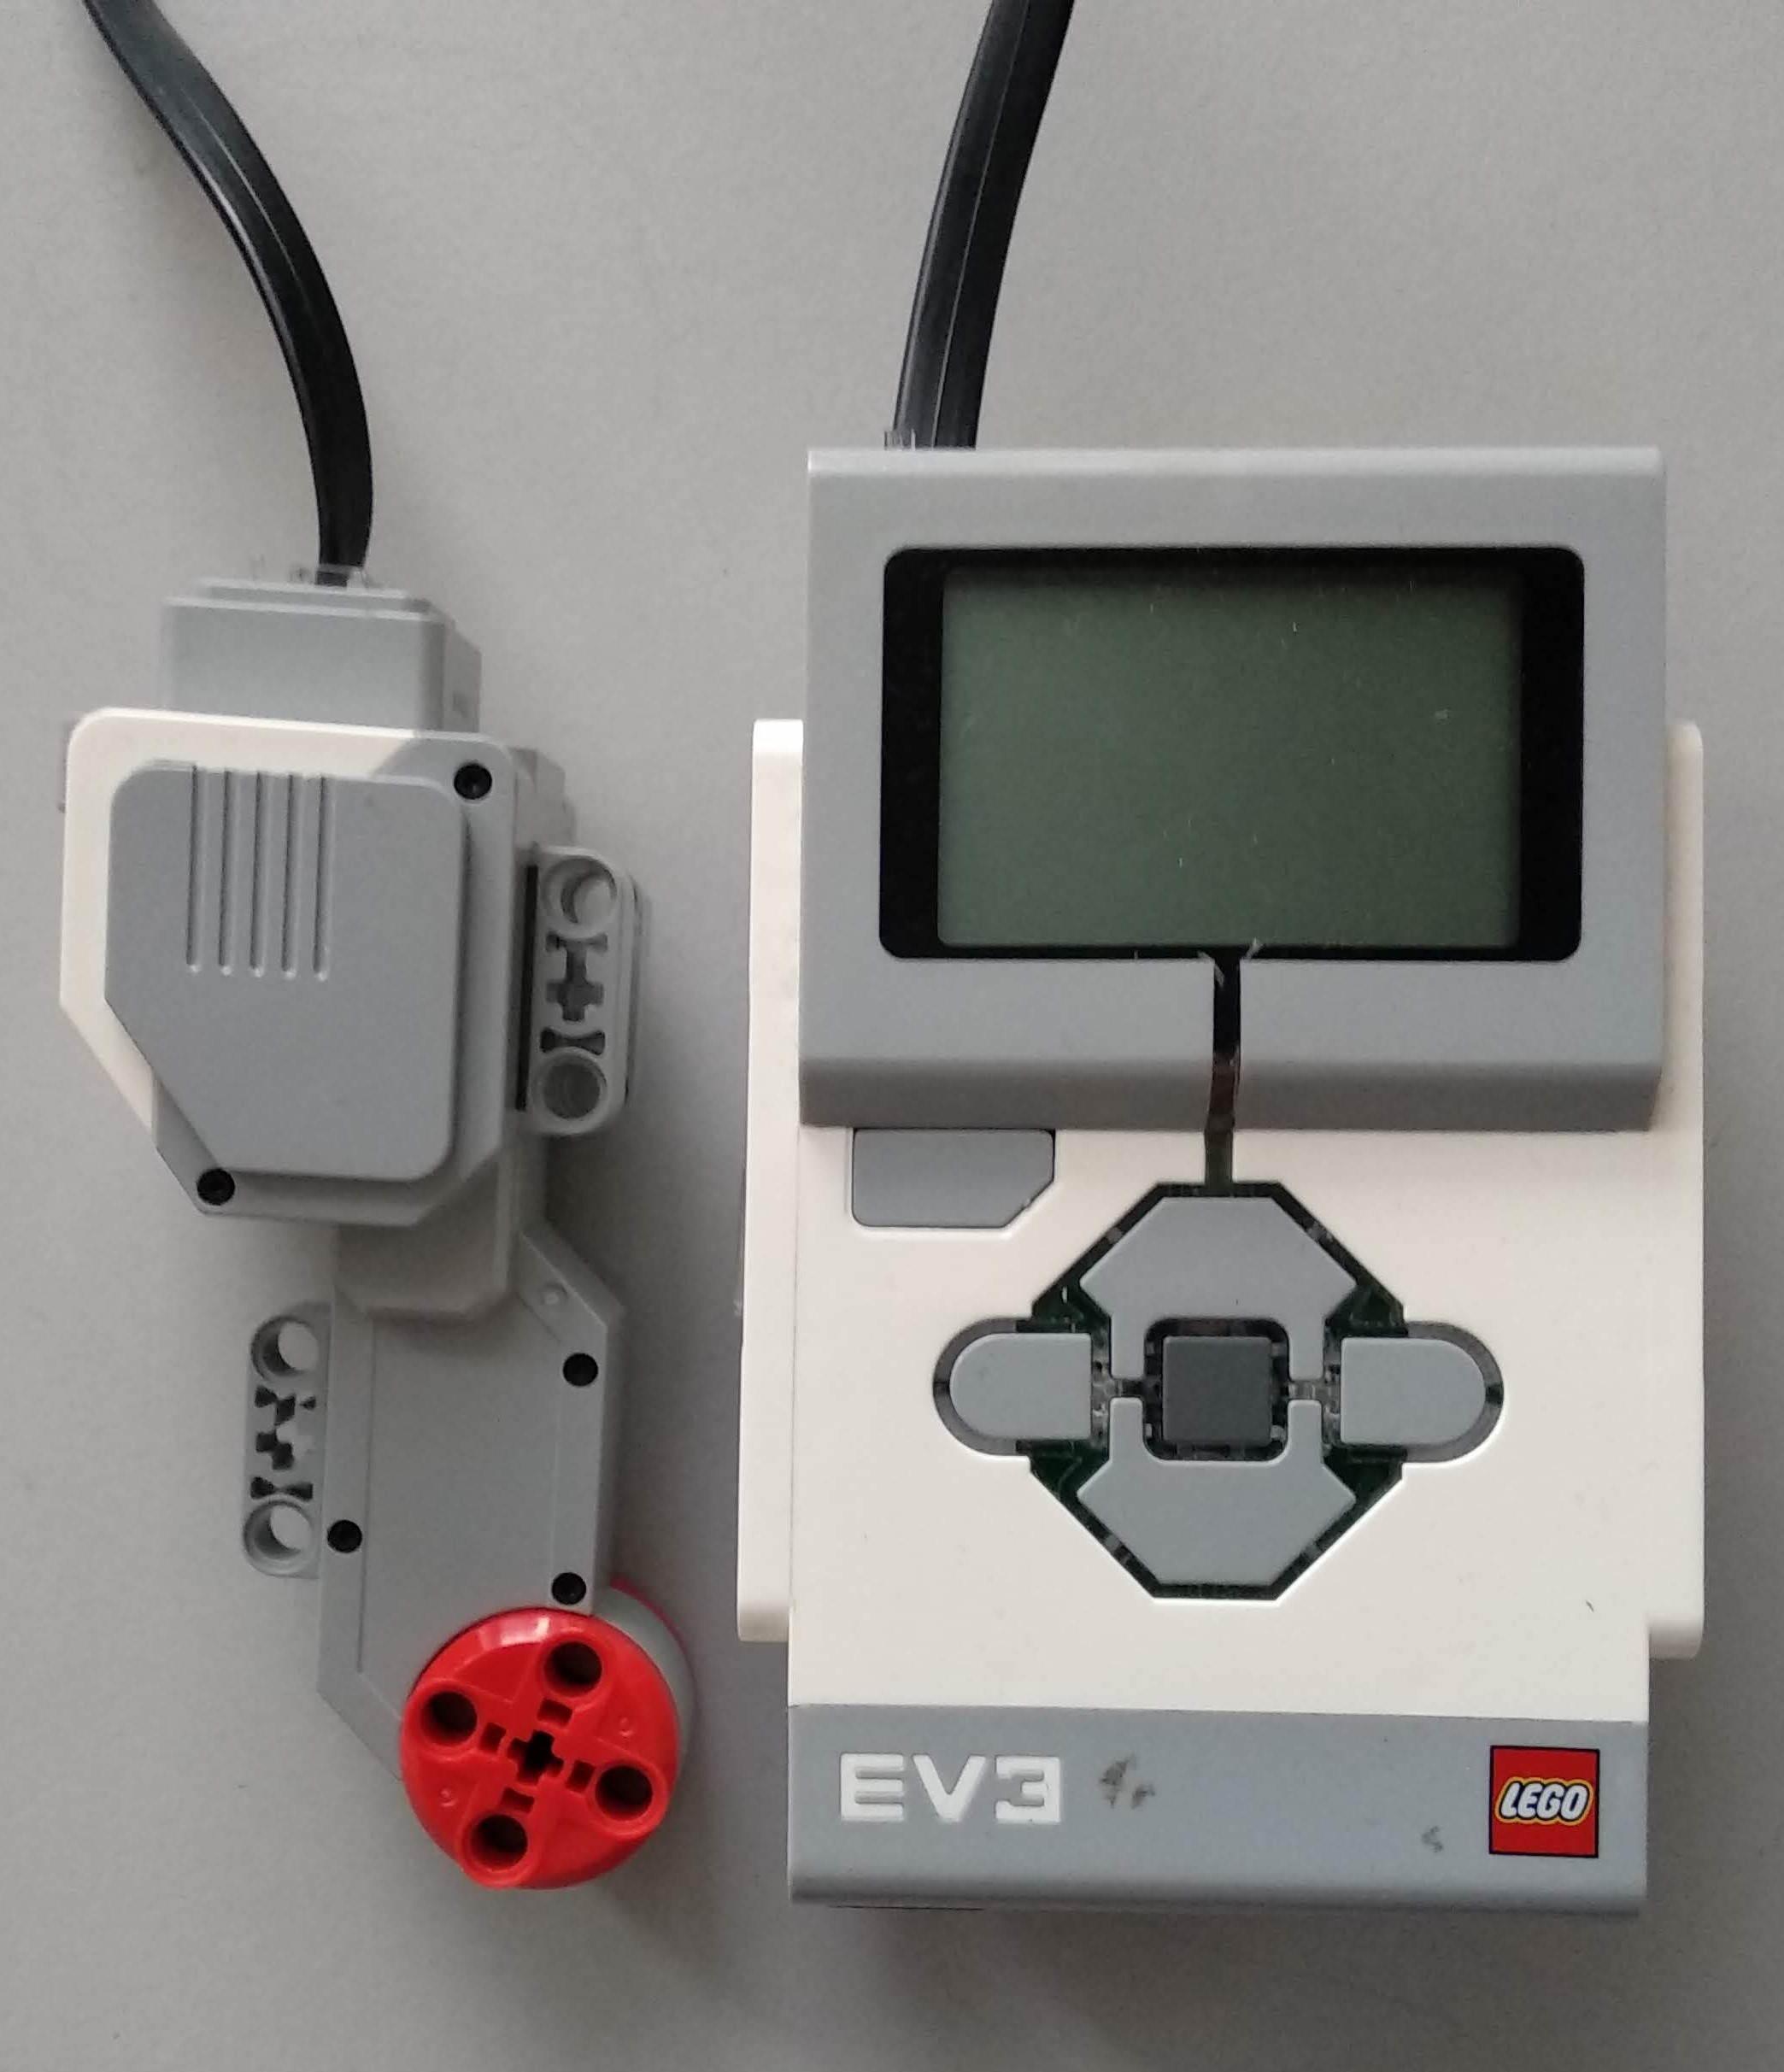
\includegraphics[scale=0.12]{Media/EV3_brick.jpg}
	}
	\caption{Общий вид экспериментальной конструкции.}
	\label{brick}
\end{figure}
\item Напишите программу, которая подает на двигатель EV3 максимально возможное постоянное напряжение (данному требованию удовлетворяет значение аргумента \verb|duty_cycle_sp| метода \verb|run_direct|, равное $100$).
При этом она также должна через одинаковые промежутки времени снимать показания текущего угла поворота ротора и записывать их вместе с соответствующими значениями времени, прошедшего с начала работы программы, в два столбца в текстовый (.txt) файл на EV3. 

Пример содержания файла (Первый столбец~--- значения угла поворота в градусах, второй столбец~--- значения времени в миллисекундах):
\begin{align*}
	&0    &&0\\
	&0    &&5\\
	&0    &&10\\
	&1    &&15\\
	&2    &&20\\
	&3    &&25\\
	&4    &&30\\
	&6    &&35\\
	&\ldots &&\ldots\\
	&391    &&491\\
	&395    &&496\\
	&400    &&501\\
	&\ldots &&\ldots
\end{align*}
\item Загрузите программу в блок EV3.
\item Запустите программу на выполнение.
\item Переместите созданный текстовый файл, содержащий экспериментальные данные, из памяти EV3 на компьютер.\label{first_file}
\item Повторите действия, описанные в трех прошлых пунктах, при 9 других значениях  аргумента \verb|duty_cycle_sp| метода \verb|run_direct|, равных элементам следующего множества $\{80, 60, 40, 20, -20, -40, -60, -80, -100\}$.\label{nine_files}
\end{enumerate}
\item Обработка экспериментальных данных.\label{scinotes_part}\\
Обработку снятых с двигателя показаний следует провести в среде Scilab. Скачать ее последнюю версию можно с сайта \mbox{\url{www.scilab.org}}.
\begin{enumerate}
\item Запустите Scilab.
 \begin{figure}[h]
	\noindent\centering{
		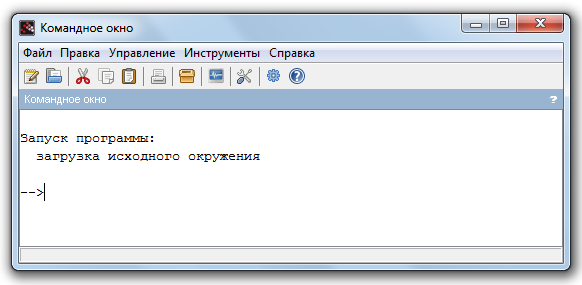
\includegraphics[scale=0.7]{Media/scilab_command_window.png}
	}
	\caption{Командное окно Scilab.}
	\label{scilab_command_window}
\end{figure}
\item В~открывшемся командном окне (рис.~\ref{scilab_command_window}) введите команду \verb|scinotes|~--- запустится редактор программного кода (рис.~\ref{scinotes_window}). Все дальнейшие действия выполняйте в данном редакторе.
\begin{figure}[h]
	\noindent\centering{
		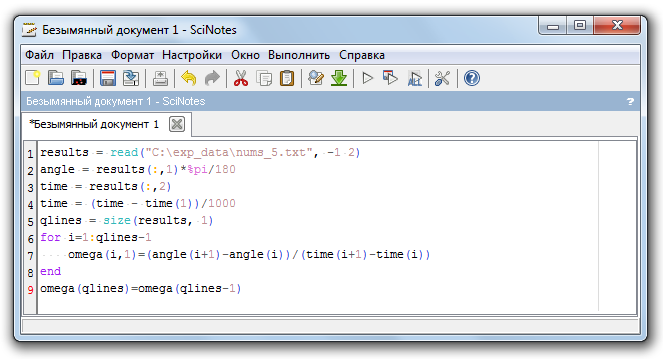
\includegraphics[scale=0.7]{Media/scinotes_window.png}
	}
	\caption{Текстовый редактор Scinotes.}
	\label{scinotes_window}
\end{figure}
\item Введите команду \verb|results=read("file_name",-1,2)|, где file\_name~--- полное имя файла, содержащего показания, снятые с двигателя во время выполнения пункта~\ref{first_file}, например C:\textbackslash Documents\textbackslash exp\_data.txt.
Функция read считывает заданный файл и на его основании формирует числовую матрицу указанного двумя последующими числами размера (первое число~--- количество строк, второе~--- столбцов). 
Число -1 ставится в том случае, если точное количество структурных единиц (столбцов или строк) неизвестно, однако писать -1 одновременно вместо двух аргументов  нельзя. 

Результат, возвращаемый этой функцией, присваивается матрице results (переменные в Scilab отдельно объявлять не надо).
\item Определите количество строк в получившейся матрице командой \verb|qlines=size(results,1)|; результат сохранится в переменной qlines. 
К~слову сказать, если взамен единицы написать 2, в переменной qlines сохранится количество столбцов.
\item Скопируйте первый столбик матрицы results в отдельную одностолбцовую матрицу angle, используя команду \verb|angle=results(:,1)|. 

Обращаясь в Scilab к отдельным элементам матриц, после имени последних в круглых скобках записывают два числа~--- соответственно номер строки и столбика, на пересечение которых находится интересующий элемент. 
Данный случай не исключение. 
Указанное на месте номера строки двоеточие означает, что обращение идет ко всем строкам сразу, поэтому в матрицу angle копируется сразу весь первый столбик.
\item Теперь переведите все значения матрицы angle из градусов в радианы: \verb|angle=angle*%pi/180|. 
Несложно догадаться, что конструкцией \verb|%pi| в Scilab обозначается число $\pi$.
\item Второй столбик матрицы results также скопируйте в отдельную одностолбцовую матрицу time и сразу же переведите из миллисекунд в секунды: \verb|time=results(:,2)/1000|. 
Одним действием можно было обойтись и в случае матрицы angle.
\item Постройте график зависимости угла поворота ротора от времени командой \verb|plot2d(time, angle, 2)|, последний аргумент которой задает цвет будущего графика.

Если теперь запустить написанный код на выполнение, кликнув, например, на изображение треугольничка на панели инструментов, то в появившемся графическом окне отобразится график, похожий на представленный на рис.~\ref{first_graph}. 

\begin{figure}[h]
	\noindent\centering{
		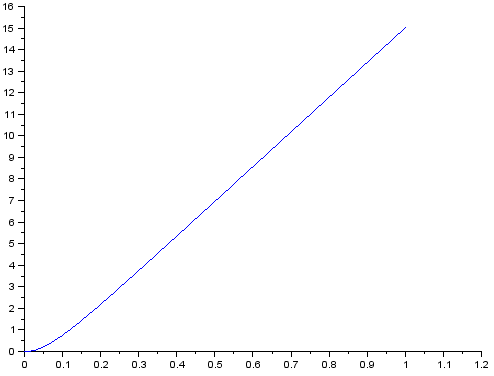
\includegraphics[scale=0.8]{Media/first_graph.png}
	}
	\caption{Первый график.}
	\label{first_graph}
\end{figure}

\item Теперь надо выполнить \textit{аппроксимацию} полученной зависимости~--- подобрать некоторую функцию и найти такое ее уравнение, которое наилучшим образом усреднит полученный результат. 
В~качестве последней следует взять непосредственно функцию $\theta(t)$~--- выражение~\eqref{theta(t)}. 
Чтобы найти \textit{методом наименьших квадратов} (прочтите о нем в дополнительной литературе) те значения параметров $\omega_{nls}$ и $T_m$, которые обеспечат графику функции~\eqref{theta(t)} наибольшее сходство с графиком, построенным на основании экспериментальных данных, в Scilab надо сделать следующее.
\begin{enumerate}
\item Сформируйте матрицу из значений функции (angle) и аргумента (time), для элементов которой необходимо выполнить аппроксимацию: \verb|aim=[time,angle]|. 
В~получившейся матрице aim первый столбец~--- матрица time, второй~--- матрица angle.

При явном определении матриц в Scilab, как в данном примере, составляющие матрицу элементы (числа или другие матрицы) после знака <<=>> записываются в квадратных [ ] или фигурных \{ \} скобках. 
Запятой разделяются элементы одной строки, а точкой с запятой (;)~--- разные строки. 

Так как матрицы time и omega одностолбцовые, то и использовался разделитель запятая. 
Таким образом они составят матрицу размером qlines$\times$2, а не столбик <<высотой>> 2qlines.
\item Транспонируйте матрицу aim: \verb|aim=aim'|.
Теперь первая ее строка~--- это матрица time, вторая~--- матрица angle. 
Такое представление матрицы aim~--- обязательное требования для правильной работы функций по аппроксимации.
\item Задайте вид функции, чьи коэффициенты будут определяться при аппроксимации. 
Для уравнения зависимости $\theta(t)$ эта операция в Scilab запишется в виде \verb|deff('e=func(k,z)','e=z(2)-k(1)*(z(1)-k(2)*(1-exp(-z(1)/k(2))))')|
На самом деле, данным действием задается некоторая функция func, которая вычисляет разность между вторым элементом одностолбцовой (или одностроковой) матрицы z (используются обозначения фигурирующие в определении функции) и значением функции~$\theta(t)$.
В~качестве параметров $\omega_{nls}$ и $T_m$ последней берутся значения одностолбцовой (или одностроковой) матрицы k, состоящей из двух элементов, а в качестве значения аргумента (времени)~--- значение первого элемента матрицы z. 

Смысл именно такого определения интересующей функции вытекает исключительно из алгоритмов, которые использует Scilab для выполнения этой операции, но о них в данном пособии говорится не будет.
\item Задайте одностолбцовую (нельзя одностроковую) матрицу att из двух элементов, где надо разместить те значения параметров $\omega_{nls}$ и $T_m$, которые, как вы думаете, получатся. 
Это помогает лишь ускорить процесс, поэтому содержание данной матрицы может быть любым, например \verb|att=[15;0.06]|.  
\item Запустите процесс аппроксимации командой \verb|[koeffs,errs] = |$\phantom{\text{datafit(func,aim,att)}}$ \verb|datafit(func,aim,att)|. 
В~результате ее работы будет создана матрица koeffs, в которую будут сохранены найденные параметры аппроксимирующей функции, и переменная errs, представляющая из себя сумму квадратов разностей экспериментального значения функции (angle) и найденного из уравнения аппроксимирующей функции для каждого из значений матрицы time.

Процесс аппроксимации может занять некоторое время.
\item Введите две новые переменные Wnls и Tm, в которые следует сохранить найденные значения параметров $\omega_{nls}$ и $T_m$ аппроксимирующей функции:
\begin{verbatim}
Wnls = koeffs(1);
Tm = koeffs(2);
\end{verbatim}
\item Для каждого из элементов матрицы time по уравнению аппроксимирующей функции определите соответствующие ее значения и заполните ими новую матрицу model посредством команды \verb|model=Wnls*(time-Tm*(1-exp(-time/Tm)))|.
\end{enumerate}
\item Постройте полученый аппроксимирующий полином, введя команду \verb|plot2d(time,model,3)|. 
Теперь весь написанный код следует запустить на выполнение.
В~результате всех проделанных действий в графическом окне появится еще одна кривая, и общий его вид станет похожим на представленный на рис.~\ref{second_graph} пример\lefteqn{.}\footnote{На представленных картинках получающиеся графики для наглядности несколько разнесены относительно друг друга. На самом же деле они будут почти полностью накладываться.} 

\begin{figure}[h]
	\noindent\centering{
		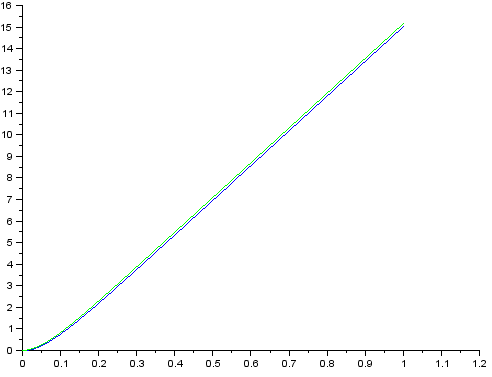
\includegraphics[scale=0.8]{Media/second_graph.png}
	}
	\caption{График с аппроксимирующей кривой.}
	\label{second_graph}
\end{figure}
\end{enumerate}
\item Моделирование схемы в Xcos.\label{xcos_part}\\
Удостовериться в том, что моделирование представленной на рис.~\ref{struct_sheme_theta} схемы исследуемого процесса дает те же результаты, что и решение дифференциальных уравнений, можно, сравнив график аппроксимирующей функции, найденной в прошлом пункте, с графиком, построенным на основании результатов моделирования схемы. 
Для создания последней следует использовать пакет прикладных математических программ для моделирования динамических систем Xcos (предустановлен в Scilab). 
Его внешний вид показан на рис.~\ref{xcos_window}.
\begin{enumerate}
\item Вызовите рабочие окна Xcos, введя в командное окно Scilab команду \verb|xcos|. 
В~случае, если не появилось окно с палитрами блоков, откройте его, пройдя в главном окне Xcos по вкладке <<Вид>> и выбрав пункт <<Палитры блоков>>. 
\item Соберите ту схему нашего двигателя, которая снабжена дополнительным интегратором и, следовательно, выдает значения угла поворота ротора (рис.~\ref{struct_sheme_theta}). 
Значения блоков (надписи на них) выставляются в окне <<Ввод значений>>, появляющемся при двойном клике на блок или при нажатии сочетания клавиш Ctrl+B с предварительным выделением кликом мыши интересующего блока. 
Обратите внимание на то, что, если вы хотите использовать в качестве значения блока некоторую переменную, предварительно ее нужно определить, введя в командном окне Scilab конструкцию типа <<имя\_переменной = ее\_значение>> (например, \verb|J = 0.0023|). 

Значение момента инерции ротора примите равным $0.0023$ (оно будет получено на следующем занятии).
Пусковой момент следует определить по формуле~\eqref{T_m}. 

\begin{figure}[h]
	\noindent\centering{
		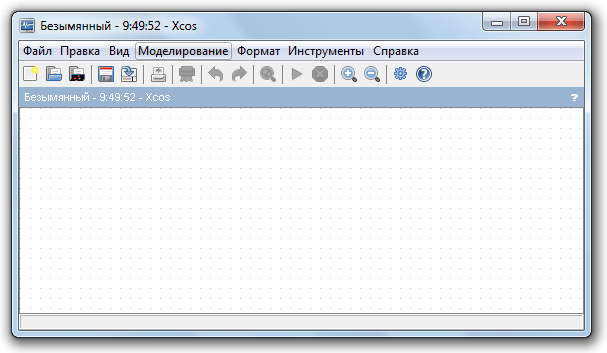
\includegraphics[scale=0.6]{Media/xcos_window.png}
	}
	\caption{Главное окно Xcos.}
	\label{xcos_window}
\end{figure}
\item В~окне <<Ввод значений>> блока с изображением часов полю <<Inizialization time>>  присвойте значение, равное нулю (в таком случае учет данных будет производиться с самого начала процесса моделирования). 
Значение второго поля (<<Period>>) есть значение упомянутой в теоретической части пособия величины $\tau$\!.
Несложно догадаться, что оно отразится лишь на плавности будущего графика, поэтому со значением $\tau$ можно поэкспериментировать.
\item \label{name} В~окне <<Ввод значений>> блока c надписью <<To workplace>> есть поле  <<Size of buffer>>, устанавливающее размер буфера для записи результатов моделирования. 
Присвойте ему значение 512. Если в дальнейшем окажется, что этого недостаточно (грубо говоря, будет отсутствовать часть графика), поменяйте установленное значение на большее. 
Имя переменной, указанное в поле <<Scilab variable name>>, есть общая часть имени массивов результатов моделирования~--- массива значений скорости (имя.values) и массива соответствующих моментов времени (имя.time). 
Значение поля <<Inherit>> оставьте равным нулю.

\begin{figure}[h]
	\noindent\centering{
		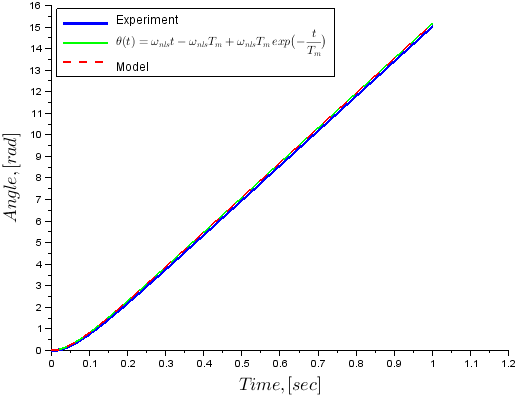
\includegraphics[scale=0.9]{Media/third_graph.png}
	}
	\caption{Итог всех построений.}
	\label{third_graph}
\end{figure}
\item Пройдите по вкладке <<Моделирование>> и выберите пункт <<Параметры>>.
В~появившемся окне полю <<Конечное время интегрирования>> присвойте значение, приблизительно равное наибольшему значению времени из графиков, построенных в прошлом пункте (<<Обработка данных>>). 
Например, на основании графиков, показанных на рис.~\ref{first_graph} и \ref{second_graph}, это значение можно принять равным $1\text{ c}$. 
\item Осуществите моделирование системы, нажав на значок с изображением треугольника или выбрав команду <<Выполнить>> во вкладке <<Моделирование>>.
\item Постройте получившийся график, дав в главном окне Scilab команду \verb|plot2d(имя.time, имя.values, 5)| (смысл <<имени>> см.~пункт~\ref{name}). 

Прежде, чем сохранять и экспортировать график в картинку, пройдите по вкладке <<Правка>>, выберете пункт <<Свойства графического окна...>> и в появившемся окне отредактируйте свойства графиков, осей и графического окна такие, как цвет, подписи к осям и~т.д. 
Пример конечного результата см.~рис.~\ref{third_graph}. Имеющаяся на нем легенда строится командой \verb|legend()|, в качестве аргументов которой следует указать названия графиков в порядке их построения и <<номер>> угла, в которой ее следует разместить. Например, показанная на рис.~\ref{third_graph} легенда была построена командой \verb|legend('Experiment','$\theta(t)=\omega_{nls}t-\omega_{nls}T_m+|\\
\verb|\omega_{nls}T_m\,exp\bigl(-\frac{t}{T_m}\bigr)$','Model',2)|\lefteqn{.}\footnote{Как видно из этой строки, чтобы применять в надписях, встречающихся в среде Scilab, команды языка \TeX\, и макропакета \LaTeX, их надо ограждать символами \$.}
\end{enumerate}
\item Повторите все описанные действия для оставшихся 9 файлов с данными, полученных в п.~\ref{nine_files} -- получите еще 9 пар значений для величин $\omega_{lns}$ и $T_m$ и 9 графиков, подобных показанному на рис.~\ref{third_graph}.
\item Постройте графики для полученных зависимостей $\omega_{lns}(\mathrm{voltage})$ и $T_m(\mathrm{voltage})$, подобные показанным на рис.~\ref{omega_nls_power} и~\ref{Tm_power}.
\begin{figure}[h!]
	\noindent\centering{
		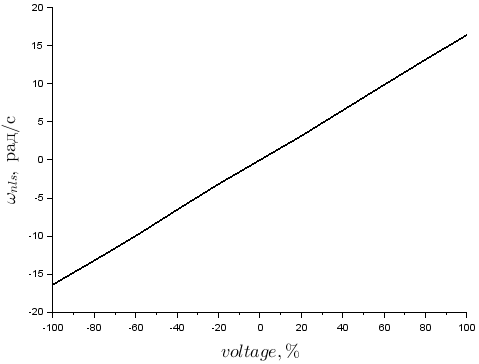
\includegraphics[scale=0.9]{Media/omega_nls_power.png}
	}
	\caption{График зависимости $\omega_{lns}(\mathrm{voltage})$.}
	\label{omega_nls_power}
\end{figure}
\begin{figure}[h!]
	\noindent\centering{
		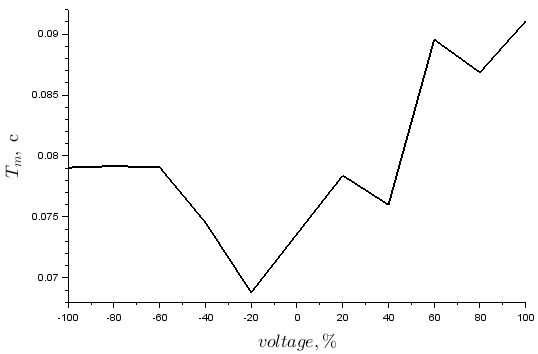
\includegraphics[scale=0.9]{Media/Tm_power.png}
	}
	\caption{График зависимости $T_m(\mathrm{voltage})$.}
	\label{Tm_power}
\end{figure}
\end{enumerate}

Любые отступления от приведенного порядка действий в рамках тех же самых программ, дающие необходимый конечный результат, разрешены.
 
\newpage 
\section{Содержание отчета}
\hspace*{\parindent}В~отчете обязательно должны присутствовать:
\begin{enumerate}
\item Графики и результаты расчетов величин $\omega_{nls}$ и $T_m$, предусмотренные пунктами~\ref{scinotes_part} и~\ref{xcos_part} раздела <<Порядок выполнения работы>>.
\item Исходный код основной расчетной программы, подготовленный с помощью редактора scinotes.
\item Построенная в Xcos схема моделирования работы двигателя EV3.
\item Исходный код написанной для EV3 программы.
\item Выводы о проделанной работе.
\end{enumerate}
\section{Приложение \\Описание метода работы с Lego EV3} \label{addition}
\subsection{Синхронизация блока EV3 и ПК по USB}
\subsubsection{Windows} 

\begin{enumerate}
\item После соединения компьютера и робота USB кабелем, пройти в Устройства и принтеры в настройках компьютера. EV3 должен быть указан как Remote NDIS Compatible Device.
\item Далее, зайти в <<Центр управления сетями и общим доступом>>, перейти во вкладку <<Изменение параметров адаптера>>. В ней среди сприска подключений можно найти EV3 подписаный как NDIS Compatible Device и ваше стандартное подключение (рис. ~\ref{Network_connections}). 

\begin{figure}[h!]
	\noindent\centering{
		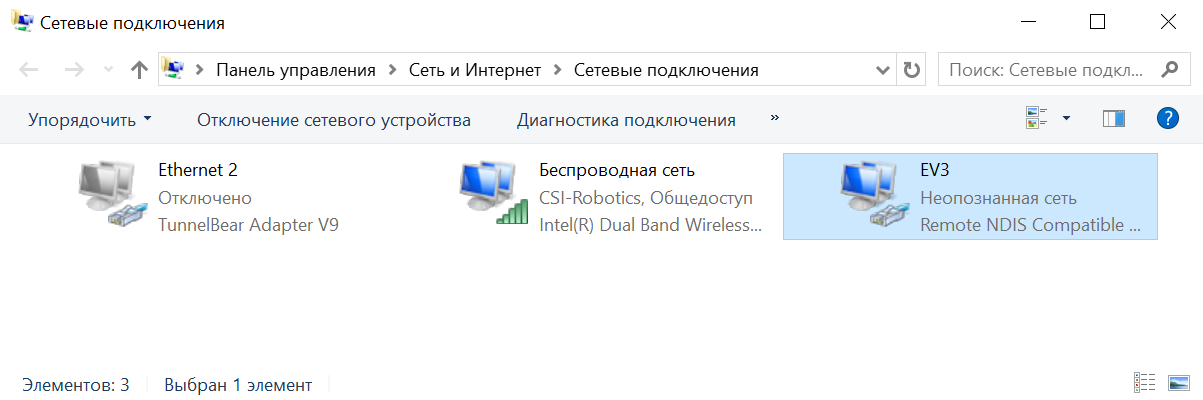
\includegraphics[scale=0.6]{Media/Network_connections.png}
	}
	\caption{Окно <<Сетевые подключения>>.}
	\label{Network_connections}
\end{figure}

\item Окрыть ваше стандартное подключение и перейти в свойства на вкладку доступ. Поставить галочку напротив <<Разрешиь другим пользователям сети использовать подключение к интернету данного компьютера>> (рис. ~\ref{Properties}).

\begin{figure}[h]
	\noindent\centering{
		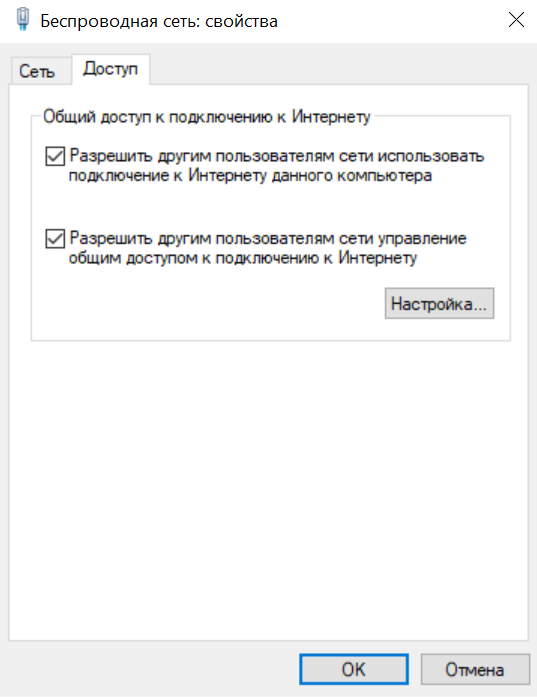
\includegraphics[scale=0.5]{Media/Properties.png}
	}
	\caption{Окно настройки доступа.}
	\label{Properties}
\end{figure}

\item После этого уже в роботе нужно зайти в Wireless and Network, далее в All Network Connections, там должно отобразиться подключение Wired. Собственно его и нужно подключить.

\begin{figure}[h!]
	\noindent\centering{
		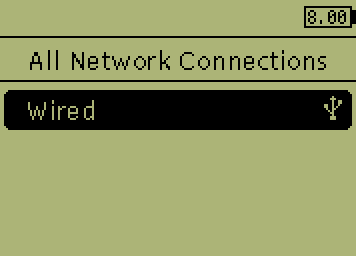
\includegraphics[scale=0.5]{Media/networking-connections-wired-only.png}
	}
	\caption{Окно EV3 <<All Network Connections>>.}
	\label{networking_EV3}
\end{figure}

\end{enumerate}

\subsubsection{Linux}

\begin{enumerate}
\item После подключения робота по USB к компьютеру, жмем на символ подключения и выбираем <<изменить соединения...>>  (рис. ~\ref{network_window}).
    
\begin{figure}[h!]
	\noindent\centering{
		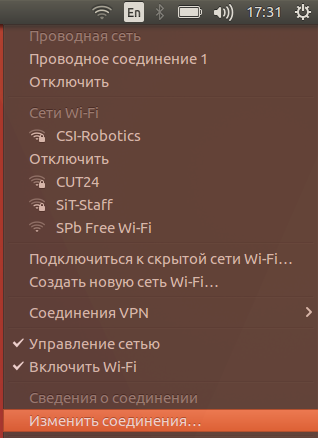
\includegraphics[scale=0.5]{Media/network_window.png}
	}
	\caption{}
	\label{network_window}
\end{figure}

\item В диалоговом окне <<Сетевые соединения>> нажать кнопку добавить, выбрать тип соединения Ethernet.

\item Откроется окно <<Изменение>>. Заполнить строку названия соединения. В строке <<Устройство>> выбрать предоставленный вам вариант и оставить только номер, как показанно на рис. ~\ref{editing_ev3_1}. 

\begin{figure}[h!]
	\noindent\centering{
		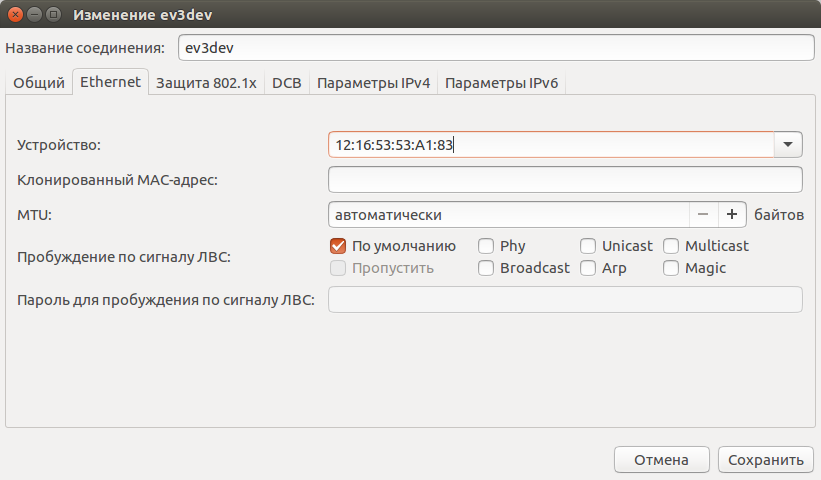
\includegraphics[scale=0.3]{Media/editing_ev3_1.png}
	}
	\caption{}
	\label{editing_ev3_1}
\end{figure}

\item Далее перейти во вкладку <<Параметры IPv4>> и выбрать способ настройки <<Предоставить сеть другим компьютерам>> (рис ~\ref{editing_ev3_2}).
  
\begin{figure}[h!]
	\noindent\centering{
		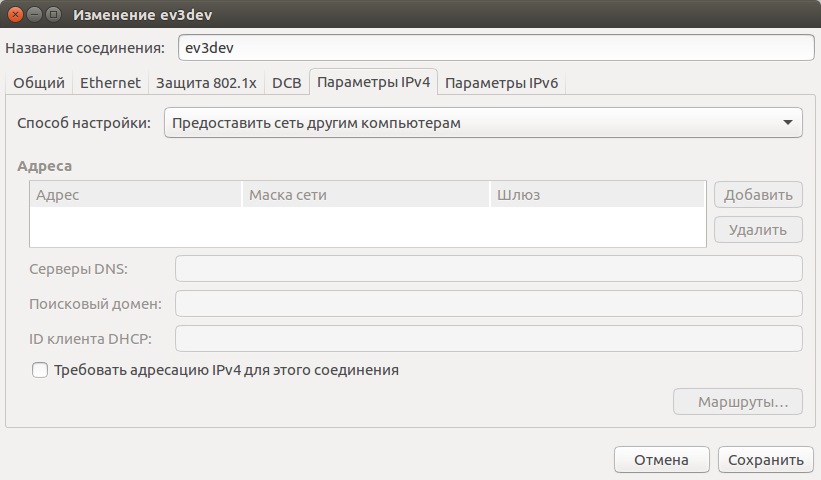
\includegraphics[scale=0.3]{Media/editing_ev3_2.png}
	}
	\caption{}
	\label{editing_ev3_2}
\end{figure}  

\item После этого уже в роботе нужно зайти в Wireless and Network, далее в All Network Connections, там должно отобразиться подключение Wired. Собственно его и нужно подключить.

\begin{figure}[h!]
	\noindent\centering{
		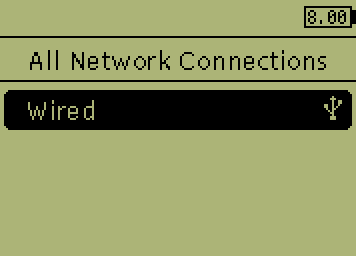
\includegraphics[scale=0.5]{Media/networking-connections-wired-only.png}
	}
	\caption{Окно EV3 <<All Network Connections>>.}
	\label{networking_EV3}
\end{figure}
    
\end{enumerate}

\subsection{Синхронизация блока EV3 и ПК по WiFi}

\hspace*{\parindent}Для того чтобы с роботом можно было работать по Wifi, необходим Wifi адаптер, вставляемый в свободное гнездо USB. 

Робот и компьютер должны быть подключены к одной и той же сети Wifi. Иных настроек не потребуется.


\subsection{Работа с файловой системой EV3}

\subsubsection{Windows}


Для работы с EV3 потребуется установить программу WinSCP.
\begin{enumerate}
\item Открываем программу WinSCP. В открывшемся диалоговом окне (рис. ~\ref{WinSCP_connection}) в качестве имени хоста используем --- \verb|ev3dev|, в качестве имени пользователя --- \verb|robot|, пароль --- \verb|maker|. Подключение можно сохранить.

\begin{figure}[h!]
	\noindent\centering{
		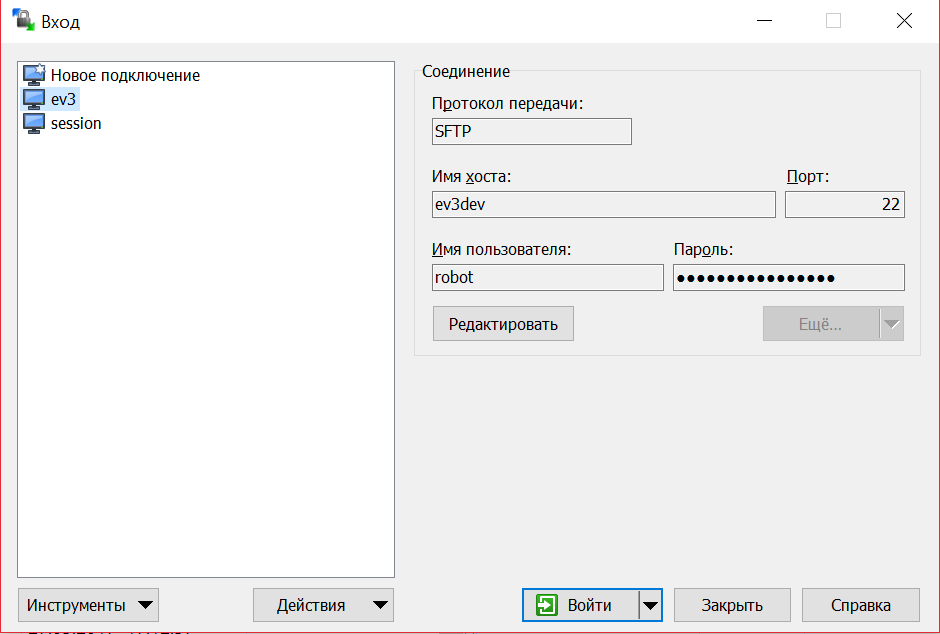
\includegraphics[scale=0.5]{Media/WinSCP_connection.png}
	}
	\caption{Окно подключения WinSCP.}
	\label{WinSCP_connection}
\end{figure}

\item Откроется окно в котором можно удобно работать с файлами внутри робота. При необходимости можно открыть консоль EV3. Метод работы с консолью робота описан ниже в п ~\ref{ev3 commands}.

\end{enumerate}

\subsubsection{Linux}
\begin{enumerate}

\itemДля начала необходимо установить на компьютер sshfs, используя команду:

\verb|sudo apt-get install sshfs|\

\item Также, необходимо создать папку, куда будет монтироваться робот:

\verb|mkdir (путь до создаваемой директории)|\

\item После чего можно начинать монтирование:

\verb|sshfs robot@(robot IP):/home/robot/ /(созданная директория)|\

\item Потребуется ввести пароль - <<maker>>, IP робота можно посмотреть в углу на экране EV3.

В примонтированной папке хранятся все файлы, находящиеся в памяти робота.

\item Далее подключается  SSH:

\verb|ssh robot@(robot ip)|\

\item Опять же, потребуется ввести пароль. После чего откроется терминал EV3 рис. ~\ref{terminal_ev3}.
\begin{figure}[h]
	\noindent\centering{
		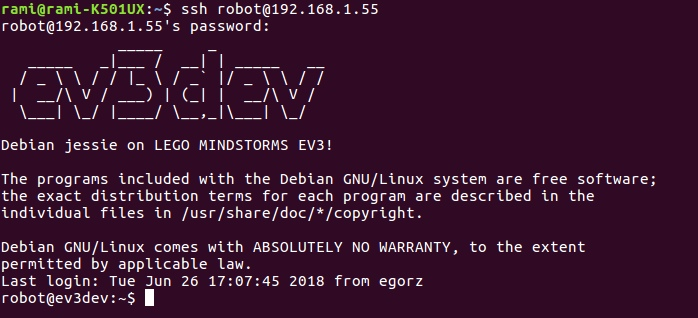
\includegraphics[scale=0.4]{Media/terminal_ev3.jpg}
	}
	\caption{Терминрал EV3}
	\label{terminal_ev3}
\end{figure}
Через этот терминал осуществляется работа с программами.
\item Для того чтобы дать роботу права на выполнение программы:\label{ev3 commands}

\verb|chmod +x file.py|\

\item Чтобы запустить программу:

\verb|./file.py|\

\item Важно! Перед завершением работы и выключением робота необходимо выключить SSH и отмонтировать папку подключённую по SSHFS.

\item Для отключения SSH достаточно ввести в терминале команду:

\verb|exit|\

\item Разрыв соединения между компьютером и роботом необходимо производить непосредственно из примонтированной папки. Для этого заходим в эту папку и, после нажатия правой кнопки мыши, выбираем пункт \verb|Открыть в терминале|. После чего вводим:

\verb|sudo umount (имя папки)|\

 Потребуется ввести пароль, после чего папка отмонтируется. EV3 можно выключать.
\end{enumerate}

\subsection{Используемые функции}
\hspace*{\parindent}При написании программы для EV3 потребутеся использовать некотрые классы и функции библиотеки EV3 и встроенные элменты языка Python.


Для импорта библиотеки EV3 необходимо прописать в начале программы следующую строку\\
\begin{itemize}
\item \verb|from ev3dev.ev3 import *|\\
Символ * в данном случае означает, что мы импортируем все элементы находящиеся в библиотеке EV3.

\item \verb|import time|\\
Подключает модуль time предназначенный для работы со временем в Python.

\item \verb|time.sleep(x)|\\
Даёт возможность приостановить выполнение программы на определенное количество секунд. Количество времени указывается вместо x. 

\item \verb|time.time()|\\
Отображеn в секундах Unix-время.  

\item \verb|mA=LargeMotor('port')|\\
Данный класс предназначен для работы с большим мотором  Lego EV3.
\\Выходные порты указываются соответствующими заглавными буквами с префиксной конструкцией out. 
Например, при подстановке в эту функцию выражения outA, в движение будет приведен двигатель, включенный в порты A. 
 
\item \verb|f = open('text.txt', 'w')|\\
Функция open открывает файл в который будет производиться запись данных
\item \verb| f.write('0'+' '+'0'+'\n')|\\
Запись в файл происходит с помощью метода write.\\
\item \verb| mA.run_direct(duty_cycle_sp=-100)|\\
Метод run direct запускает мотор с коэффициентом заполнения определённым duty cycle sp в пределах от -100 до 100.\\
Коэффициент заполнения --- это отношение длительности импульса к периоду импульса. 
\item \verb|mA.position|\\
position метод возвращающий угол поворота двигателя.

\end{itemize}

\end{document}
